% vim:set shiftwidth=2 tabstop=2 expandtab:

\chapter{Nonlinear Parametric Cointegration Model} \la{chap:6}
\ifpdf
    \graphicspath{{Chapter6/Chapter6Figs/PNG/}{Chapter6/Chapter6Figs/PDF/}{Chapter6/Chapter6Figs/}}
\else
    \graphicspath{{Chapter6/Chapter6Figs/EPS/}{Chapter6/Chapter6Figs/}}
\fi

 In this chapter we extend from nonparametric estimation methods to parametric approch. We develop asymptotic theory for a nonlinear parametric cointegrating regression model. We establish a general framework for  weak consistency that is easy to apply for various nonstationary time series, including partial sum of linear processes and  Harris recurrent Markov chains. We provide  limit distributions for  nonlinear least squares  estimators,    extending the previous work.  We also introduce endogeneity to the model by allowing the error to be serially dependent and cross correlated with the regressors.



\section{Introduction} \la{sec:6:intro}
Consider a typical nonlinear parametric cointegrating regression model has the form
 \be y_t&=&
f(x_t, \theta_0)+\,  u_t, \quad t=1,...,n,\la {intro.eqn1}
\ee
where  $f:\mathbb{R} \times \mathbb{R}^m \rightarrow \mathbb{R}$ is a known nonlinear function,
$x_t$ and  $u_t$ are regressor and regression errors, and   $\theta_0$ is an $m$-dimensional true parameter vector that lies in the parameter set $\Theta$. With the observed nonstationary data $\{y_t, x_t\}_{t=1}^n$, this paper is concerned with the nonlinear least squares (NLS) estimation of the unknown parameters $\theta\in \Theta$. In this regard, \cite{parkphillips2001} (PP henceforth) considered $x_t$ to be an integrated, $I(1)$, process. Based on PP framework, \cite{changparkphillips2001} introduced additional linear time trend term and stationary regressors into model (\ref{intro.eqn1}). \cite{changpark2003} extended to nonlinear index models driven by integrated processes.  More recently, \cite{choisaikkonen2010}, \cite{gaokinglutjostheim2009} and \cite{wangphillips2012} developed statistical tests  for the existence of a nonlinear cointegrating relation. \cite{changpark2010} allowed the regressors $x_t$ to be contemporaneously correlated with the regression errors $u_t$ and \cite{shiphillips2010} extended the model (\ref{intro.eqn1}) by incorporating a loading coefficient.


The present chapter has a similar goal to the previously mentioned papers but offers more general results, which have some advantages for empirical studies. First of all, we establish a general framework for  weak consistency of the NLS estimator $\hat{\theta}_n$, allowing for the $x_t$ to be  a  wider class of nonstationary time series.
 The set of sufficient conditions are easy to apply to various nonstationary regressors, including partial sum of linear processes and recurrent Markov chains. Furthermore, we  provide limit distributions for the NLS estimator $\hat{\theta}_n$. It  deserves to mention that  the routine employed in this chapter to establish the limit distributions of $\hat\theta_n$ is different from those used in the previous works, e.g. PP. Roughly speaking, our routine is related to joint distributional convergence of a martingale under target and its conditional variance, rather than using classical martingale limit theorem which requires establishing the convergence in probability for the conditional variance.  In nonlinear cointegrating regressions, there are   some advantages for our methodology  since it is usually difficult to establish the convergence in probability for the conditional variance, in particular, in the situation that the regressor $x_t$ is a nonstationary time series.
Second, in addition to the commonly used martingale innovation structure, our model allows for serial dependence in the equilibrium errors $u_t$ and the innovations driving $x_t$. It is important as our model  permits joint determination of $x_t$ and $y_t$, and hence the system is a time series structural model. Under such situation, the weak consistency and limit distributions of the NLS estimator $\hat{\theta}_n$ are also established.

This chapter is organized as follow. Section \ref{sec:6:weakConsistency} presents our main results on weak consistency of the NLS estimator $\hat \theta_n$. Theorem \ref{thmConsistency} provides a general framework.  Its applications to integrable and non-integrable $f$  are given in Theorems \ref{thmLinearConsistency}--\ref{thmHomoConsistent1}, respectively.  \ref{sec:6:limitDistribution} investigates the limit distributions of $\hat \theta_n$ in which the model (\ref {intro.eqn1}) has a martingale structure. Extension to endogeneity is presented in Section \ref{sec:6:endo}. As mentioned above, 
our routine establishing the limit distribution of $\hat \theta_n$ is different from previous works. Section \ref{sec:6:simulation} performs simulation,  reporting and discussing the numerical values of means and standard errors which provide the evidence of accuracies of our NLS estimator. Section \ref{sec:6:example} presents  an empirical example,  providing a link between our theory and real applications. The model of interest is the carbon Kuznets curve relating the per capita CO$_2$ emissions and per capita GDP. Endogeneity occurs in this example due to potential misreporting of GDP, omitted variable bias and reverse causality. Section \ref{sec:6:conclusion} concludes the paper. Technical proofs are postponed to Section \ref{sec:6:proof}.

Throughout the chapter, we denote constants by $C, C_1, C_2,...$ which may be different at each appearance. For a vector $x=(x_1,...,x_m)$, assume that $\|x\|=(x_1^2+...+x_m^2)^{1/2}$, and for a matrix $A$, the norm operator $\|\cdot\|$ is defined by $\|A\| =\sup_{x: \|x\| = 1} \|xA\|$. Furthermore,  the parameter set $\Theta \subset \mathbb {R}^m$ is assumed to be compact and convex, and the true parameter vector $\theta_0$ is an interior point of $\Theta$.


\section {Weak consistency} \la{sec:6:weakConsistency}

This section considers the estimation of the unknown parameters $\theta$ in model (\ref {intro.eqn1}) by NLS.
Let $Q_n(\theta) = \sum_{t = 1}^n ( y_t - f(x_t, \theta))^2$. The NLS estimator $\hat\theta_n$ of $\theta$
is defined to be the minimizer of $Q_n(\theta)$ over $\theta \in \Theta$, that is,
\be
\hat{\theta}_n = \arg{\min}_{\theta \in \Theta} Q_n(\theta) , \la {sad2}
\ee
and the error estimator is defined by $\hat{\si}_n^2 = n^{-1} \sum_{t = 1}^n \hat{u}_t^2$, where $\hat{u}_t = y_t - f(x_t, \hat{\theta}_n)$. To investigate the weak consistency for the NLS estimator $\hat\theta_n$,
this section assumes the  regression model (\ref {intro.eqn1}) to have a martingale structure.
In this situation, our sufficient conditions are  closely related  to those of \cite{wu1981}, \cite{lai1994} and \cite{skouras2000}, and they intend  to provide a general framework. In comparison to the papers mentioned, our assumptions are easy to apply, particularly in nonlinear cointegrating regression situation as stated in the two examples below. Extension to endogeneity between $x_t$ and $u_t$ is investigated in Section \ref{sec:6:endo}.

\subsection{A framework} \la{sec:6:framework}

We make use of the following assumptions for the development of the weak consistency.

\begin{assump} \la{assumpClose}
For each $\pi,\pi_0 \in \Theta$, there exists a real function $T:\mathbb{R} \rightarrow \mathbb{R}$ such that
\be
|f(x, \pi) - f(x, \pi_0)| \le h(||\pi - \pi_0||) \,T(x), \la {45}
 \ee
 where $h(x)$ is a bounded real function such that $h(x)\downarrow h(0)=0$, as $x\downarrow 0.$
\end{assump}

\begin{assump} \la{assumpMartingale}
\begin{enumerate}[label=(\roman{*}), leftmargin=*, widest=0] \itemsep0pt \parskip0pt \parsep0pt
\item $\{u_{t},\mathcal{F}_{t},1\leq t\leq n\}$ is a martingale
difference sequence satisfying
$E(|u_t|^2|\mathcal{F}_{t-1}) = \si^2$ and $\sup_{1\leq t\leq n}E(|u_{t}|^{2q}|\mathcal{F}_{t-1})<\infty$ a.s., where $q > 1$; and
\item $x_t$ is adapted to $\F_{t - 1}$, $t = 1, ..., n$.
\end{enumerate}
\end{assump}

\begin{assump} \la {assumpLowerBound} There exists an increasing sequence $0<\kappa_n \to \infty$ such that
 \be\kappa_n^{-2} \sum_{t = 1}^n [T(x_t) + T^2(x_t)] = O_P(1), \la{20}\ee and for any $0<\eta<1$ and $\theta \ne \theta_0$, where $\theta, \theta_0\in \Theta$, there exist
 $n_0 > 0$ and $M_1>0$ such that
\be
P \Big ( \sum_{t = 1}^n ( f(x_t, \theta) - f(x_t, \theta_0))^2 \ge \kappa_n^2\,/ M_1 \Big ) \ge 1 - \eta, \la {21}
\ee
 for   all $n > n_0$.
\end{assump}

\begin{thm} \la{thmConsistency} Under Assumptions \ref{assumpClose}--\ref{assumpLowerBound}, the NLS estimator $\hat{\theta}_n$ is a consistent estimator of $\theta_0$, i.e. $\hat{\theta}_n \rightarrow_P \theta_0$.
If in addition $\kappa_n^2 n^{-1} = O(1)$, then $\hat{\si}^2_n \to_P \si^2$, as $n \to \infty$.
\end{thm}


Assumptions \ref {assumpClose} and \ref{assumpMartingale} are the same as those used in \cite{skouras2000}, which are standard in the NLS estimation theory. Also see \cite{wu1981} and \cite{lai1994}. Assumption \ref {assumpLowerBound} is used to replace (3.8), (3.9) and (3.11) in \cite{skouras2000}, in which some uniform conditions are used. In comparison to \cite{skouras2000}, our Assumption \ref {assumpLowerBound} is related to the conditions on the regressor $x_t$ and is more natural and easy to apply. In particular, it is directly applicable in the situation that $T$ is integrable and the regressor $x_t$ is a nonstationary time series, as stated in the following sub-section.

\subsection{Identification of Assumption \ref{assumpLowerBound}: integrable functions } \la{sec:6:consistencyIntegrable}
Due to Assumption \ref{assumpClose}, $f(x, \theta)-f(x, \theta_0)$ is integrable in $x$ if $T$ is an integrable function. This class of functions includes $f(x, \theta_1, \theta_2)=\theta_1 |x|^{\theta_2}I(x\in [a, b])$, where $a$ and $b$ are finite constants,  the Gaussian function $f(x, \theta) = e^{-\theta x^2}$, the Laplacian function $f(x, \theta) = e^{-\theta |x|}$, the logistic regression function $f(x, \theta)=e^{\theta |x|}/(1+e^{\theta |x|})$,  etc. In this sub-section, two commonly used  non-stationary regressors $x_t$ are shown to satisfy Assumption \ref{assumpLowerBound} if $T(x)$ is integrable.

\medskip \noindent
{\bf Example 1 (Partial sum of linear processes).}
Let $x_{t}=\sum_{j=1}^t \xi_{j}$, where $\{\xi _{j},j\geq 1\}$ is a linear process
defined by
\begin{equation}
\xi _{j}=\sum_{k=0}^{\infty }\,\phi _{k}\,\epsilon _{j-k}, \la {sec2.f1}
\end{equation}
where $\{\epsilon _{j},-\infty <j<\infty \}$ is a sequence of i.i.d.
random variables with $E\epsilon _{0}=0$, $E\epsilon _{0}^{2}=1$ and the
characteristic function $\varphi (t)$ of $\epsilon _{0}$ satisfying
$\int_{-\infty }^{\infty }|\varphi (t)|dt<\infty $.
The coefficients $\phi_k$ are assumed to satisfy one of the following conditions:

{\textbf{C1.}} $\phi_k \sim  k^{-\mu} \rho(k)$, where $1 / 2 < \mu < 1$ and $\rho(k)$ is a function slowly varying at $\infty$.

{\textbf{C2.}} $\sum_{k=0}^{\infty }k|\phi _{k}|<\infty $ and $\phi \equiv \sum_{k=0}^{\infty }\phi_{k}\not =0$.

\noindent Put $d_n^2 = \E x_n^2.$ As in \cite{wanglingulati2003}, we have
\be
d_n^2 = \E x_n^2 \sim
\begin{cases}
c_{\mu} n^{3-2\mu} \rho^2(n),  & \mbox{under {\bf C1},} \\
\phi^2 n, & \mbox{under {\bf C2},}
\end{cases}
\ee
where $c_\mu = 1 / ((1 - \mu)(3-2\mu )) \int_{0}^{\infty} x^{-\mu} (x+1)^{-\mu} dx$.
We have the following result.

\begin{thm} \la{thmLinearConsistency} Suppose $x_t$ is defined as in Example 1 and Assumption \ref{assumpClose} holds. Assume:
\begin{enumerate}[label=(\roman{*}), leftmargin=*] \itemsep0pt \parskip0pt \parsep0pt
\item $T$ is bounded and integrable, and
\item $\int_{-\infty}^{\infty} (f(s, \theta) - f(s, \theta_0))^2 ds>0$ for all $\theta\not=\theta_0$.
\end{enumerate}
Then (\ref {20}) and (\ref {21}) hold with $\kappa^2_n=n/d_n$.  Consequently,
if in addition  Assumption \ref{assumpMartingale}, then $\hat{\theta}_n \rightarrow_P \theta_0$.
\end{thm}

Theorem \ref{thmLinearConsistency} improves Theorem 4.1 of PP in two folds. Firstly, we allow for more general regressor. The result under {\bf C1} is new, which allows $x_t$ to be long memory process, including the fractionally integrated process as an example. PP only allow $x_t$ to satisfy {\bf C2} with additional conditions on $\phi_k$, that is, they require $x_t$ to be a partial sum of short memory process. Secondly, we remove the part (b) required in the definition of I-regular function given in their Definition 3.3. Furthermore,  we allow for certain  non-integrable $f$  such as the logistic regression function $f(x, \theta)=e^{\theta |x|}/(1+e^{\theta |x|})$, $ \theta\ge \theta_0$ for some $\theta_0>0$, although we assume the integrability of  $T$.

\medskip \noindent
{\bf Example 2  (Recurrent Markov Chain).}
Let $\{x_k\}_{k\ge 0}$ be a Harris recurrent Markov chain with state space $(E, \mathcal{E})$,
transition probability $P(x, A)$ and invariant measure $\pi$. We denote $P_\mu$ for the Markovian probability
with the initial distribution $\mu$, $E_\mu$ for correspondent expectation and $P^k(x, A)$
for the $k$-step transition of $\{x_k\}_{k\ge 0}$.  A subset $D$ of $E$ with $0<\pi(D)<\infty$ is called $D$-set of $\{x_k\}_{k\ge 0}$ if for any $A\in \mathcal{E}^+$,
$$
\sup_{x\in E} E_x\big(\sum_{k=1}^{\tau_A}I_D(x_k)\big)<\infty,
$$
where $ \mathcal{E}^+=\{A\in  \mathcal{E}: \pi(A)>0\}$ and $\tau_A=\inf\{n\ge 1: \ x_n\in A\}$. By Theorem 6.2 of \ref{orey1971},
$D$-sets not only exist,  but generate the entire sigma $\mathcal{E}$, and
 for any $D$-sets $C, D$ and any probability measure $\nu, \mu$ on $(E, \mathcal{E})$,
\be
\lim_{n\to\infty}\sum_{k=1}^n\nu P^k(C)/\sum_{k=1}^n\mu P^k(D) &=&\frac {\pi (C)}{\pi (D)}, \la {1.3}
\ee
where $\nu P^k(D) =\int_{-\infty}^{\infty} P^k(x, D)\nu(dx)$. See \cite{nummelin2004} for instance.

Let a $D$-set $D$ and a probability measure $\nu$ on $(E, \mathcal{E})$ be fixed. Define
\bestar
a(t) &=& \pi^{-1}(D)\sum_{k=1}^{[t]}\nu P^k(D), \quad t\ge 0.
\eestar
 By recurrence, $a(t)\to\infty$. Here and below, we set the state space to be the real space, that is $(E, \mathcal{E}) = (R, \mathcal{R})$. We have the following result.

\begin{thm} \la {thmMarkovConsistency} Suppose $x_t$ is defined as in Example 2 and Assumption \ref{assumpClose} holds. Assume:
\begin{enumerate}[label=(\roman{*}), leftmargin=*] \itemsep0pt \parskip0pt \parsep0pt
\item $T$ is bounded and $\int_{-\infty}^{\infty} |T(x)|\pi(dx) < \infty$, and
\item $\int_{-\infty}^{\infty} (f(s, \theta) - f(s, \theta_0))^2 \pi(ds)>0$ for all $\theta\not=\theta_0$.
\end{enumerate}
Then (\ref {20}) and (\ref {21}) hold with $\kappa^2_n=a(n)$.  Consequently,
if in addition  Assumption \ref{assumpMartingale}, then $\hat{\theta}_n \rightarrow_P \theta_0$.

\end{thm}

Theorem \ref {thmMarkovConsistency} seems to be new to the literature. By virtue of (\ref {1.3}), the asymptotic order of $a(t)$ depends only on $\{x_k\}_{k\ge 0}$.
It is interesting to notice that Theorem \ref {thmMarkovConsistency} does not impose the $\beta$-regular condition as commonly used in the literature. The Harris recurrent Markov chain $\{x_k\}_{k\ge 0}$  is called $\beta$-regular if
\be
\lim_{\lam\to \infty} a(\lam t)/a(\lam) &=&t^\beta,\quad \forall t>0, \la {d1}
\ee
where $0< \beta\le 1$. See \cite{chen1999} for instance.


\subsection{Identification of Assumption \ref{assumpLowerBound}: beyond integrable functions} \la{sec:6:consistencyNonIntegrable}
As noticed in Section \ref{sec:6:consistencyIntegrable},  Assumption \ref{assumpLowerBound} still holds for certain non-integrable $f$, although we require the integrability of $T$. However,   identification of Assumption \ref{assumpLowerBound} is more involved for  general non-integrable $f$. In this situation, instead of requiring $T$ to be integrable, we impose certain relationship between  $f$ and $T$.

\begin{assump} \la{assumpHomo}
\begin{enumerate}[label=(\roman{*}), leftmargin=*, widest=0] \itemsep0pt \parskip0pt \parsep0pt
\item There exist a regular function\footnote{Function $H$ is called regular on $\Theta$ if (a) for all $\theta \in \Theta$, there exist for each $\epsilon > 0$ continuous functions $\underline{H}_\epsilon$, $\overline{H}_\epsilon$, and a constant $\delta_\epsilon > 0$ such that $\underline{H}_\epsilon(x, \theta) \le H(y, \theta) \le \overline{H}_\epsilon(x, \theta)$ for all $|x - y| < \delta_\epsilon$ on $K$, a compact set of $R$, and such that $\int_K (\overline{H}_\epsilon - \underline{H}_\epsilon)(x, \theta)dx \rightarrow 0$ as $\epsilon \rightarrow 0$, and
(b) for all $x \in R$, $H(x, \cdot)$ is equicontinuous in a neighborhood of $x$.
} $g(x, \theta, \theta_0)$ on $\Theta$ satisfying $$\int_{|s| \le \de} g^2(s, \theta, \theta_0) ds > 0$$  for all $\theta \ne \theta_0$ and $\de > 0$, a real function $T: \mathbb{R} \to  \mathbb{R}$ and a positive real function  $v(\lambda)$ which is bounded away from zero as $\lambda \to \infty$, such that for any bounded $x$,
\be
\sup_{\theta, \theta_0\in \Theta}|f(\lam x, \theta) - f(\lam x, \theta_0)- v(\lam)\,g(x, \theta, \theta_0)|/T(\lam x) &=&o(1),
\ee
as $\lam \to \infty$.
\item There exists a real function $T_1: \mathbb{R} \to \mathbb{R}$  such that $T(\lam x)\le v(\lam)\, T_1(x)$ as $|\lam x|\to \infty $ and $T_1+ T_1^2$ is locally integrable (i.e. integrable on any compact set).
\end{enumerate}
\end{assump}

\begin{thm} \la {thmHomoConsistency} Suppose Assumption \ref{assumpHomo} holds. Suppose that there exists a continuous Gaussian process $G(t)$ such that $x_{[nt], n} \Rightarrow G(t)$, on $D[0,1]$, where $x_{i,n} = x_i / d_n$  and $0 < d_n \to \infty$ is a sequence of real numbers.
Then (\ref {20}) and (\ref {21}) hold with $\kappa^2_n=nv^2(d_n)$. Consequently,
if in addition Assumption \ref{assumpClose} and \ref{assumpMartingale} and the assumption that the $T$'s in \ref{assumpClose} and \ref{assumpHomo} coincide,, then $\hat{\theta}_n \rightarrow_P \theta_0$.
\end{thm}


Assumptions \ref{assumpClose} and \ref{assumpHomo} are quite general, including many commonly used regression functions. Typical examples include $f(x, \theta)=(x+\theta)^2,\ \theta e^{x}/(1 + e^x),\ \theta \log |x|,\ \theta |x|^\al$ ($\al$ is fixed) and $\theta_0+\theta_1 |x|+...+\theta_k|x|^k$.
The class of functions satisfying Assumptions \ref{assumpClose} and \ref{assumpHomo} are similar to, but wider than the  $H_0$-regular functions on $\Theta$ imposed in Theorem 4.2 of PP. For instance,   Assumptions \ref{assumpClose} and \ref{assumpHomo} (hence Theorem 2.4) are applicable for   the function $f(x, \theta)=(x+\theta)^2$  [with $T(x)= T_1(x)=|x|$, $v(\lam)=\lam$ and $g(x, \theta, \theta_0)=2(\theta-\theta_0)\, x$], but Theorem 4.2 of PP is not  directly applicable for this function. See, e.g., Example 4.1 (c) of PP. We also mention that our condition on the regressor $x_t$ is much general than that of PP, as we only require that $x_{[nt]} / d_n$ converges weakly to a continuous Gaussian  process. This kind of weak convergence condition is very likely close to be necessary.

\medskip
We next consider  a class of asymptotically homogeneous functions. In this regard, we follow PP. Let $f:\mathbb{R} \times \Theta \rightarrow \mathbb{R} $ have the structure:
 \be
 f(\lambda x, \theta) = v(\lambda, \theta) h(x,\theta) + b(\lambda, \theta)\, A(x, \theta)\, B(\lambda x, \theta), \la {sad1}
 \ee
 where $\sup_{\theta\in \Theta}|b(\lambda, \theta)\, v^{-1}(\lambda, \theta)|\to 0$, as $\lambda\to \infty$; $\sup_{\theta\in \Theta}|A(x, \theta)|$ is locally bounded, that is, bounded on bounded intervals;
 $\sup_{\theta\in \Theta} |B(\lambda x, \theta)|$ is bounded on $R$; $h(x, \theta)$ is regular on $\Theta$ satisfying $\int_{|s| \le \de} h^2(s, \theta)  ds > 0$   for all $\theta \ne \theta_0$ and $\de > 0$,  and $v(\lambda, \theta)$ satisfy:   there exist $\ep > 0$ and a neighborhood $N$ of $\bar{\theta}$ such that as $\lambda \to \infty$
\be
\inf_{\substack{|p-\bar{p}| < \ep \\ |q-\bar{q}| < \ep}} \inf_{\theta \in N} |p v(\lambda, \theta) - q v(\lambda, \theta_0) | \to \infty,
\ee
for any $\bar{\theta} \ne \theta_0$ and $\bar{p}, \bar{q} > 0$.


\begin{thm} \la {thmHomoConsistent1} Suppose that $f$ in model (\ref {intro.eqn1}) has the structure (\ref {sad1}), and in addition to Assumption \ref{assumpMartingale}, there exists a continuous Gaussian process $G(t)$ such that $x_{[nt], n} \to_D G(t)$, on $D[0,1]$, where $x_{i,n} = x_i / d_n$  and $0 < d_n \to \infty$ is a sequence of real numbers. Then,
 the NLS estimator $\hat{\theta}_n$ defined by (\ref {sad2}) is a consistent estimator of $\theta_0$, i.e. $\hat{\theta}_n \rightarrow_P \theta_0$.
\end{thm}





 The conditions on $f$ given in Theorem \ref {thmHomoConsistent1} are the same as those used in Theorem 4.3 of PP, which are satisfied by the functions such as  the Box-Cox transformation $(|x|^\theta - 1)/\theta$. The difference between current Theorem \ref{thmHomoConsistent1} and Theorem 4.3 of PP is   we only require that $x_{[nt]} / d_n$ converges weakly to a continuous Gaussian  process, which  is  close to be necessary.


To investigate the weak consistency of $\hat\theta_n$, this section makes use of three conditions sets on $f$: Assumption \ref{assumpClose} with $T$ being integrable (Theorems \ref{thmLinearConsistency}--\ref{thmMarkovConsistency}); Assumptions \ref{assumpClose}--\ref{assumpHomo} (Theorem \ref{thmHomoConsistency}) and the condition (\ref {sad1}) (Theorem \ref{thmHomoConsistent1}). We remark that these conditions sets are mutually exclusive. There are examples on the $f$ such that one of these assumptions holds, but not for other two. For instance, the function $f(x, \theta)=\theta/(1+x^2)$ satisfies Assumption \ref{assumpClose}  with $h(x)=x$ and $T(x)=1/(1+x^2)$, but Assumption \ref{assumpHomo} and  the condition (\ref {sad1}) fail; the function $f(x, \theta)=(x+\theta)^2$ satisfies Assumptions \ref{assumpClose}--\ref{assumpHomo}, but not for Assumption \ref{assumpClose} with $T$ being integrable and the condition (\ref {sad1}).


\section{Limit distribution} \la{sec:6:limitDistribution}
This section considers  limit distribution of $\hat{\theta}_n$. In what follows,  let $\dot{Q}_n$ and $\ddot{Q}_n$ be the first and second derivatives of $Q_n(\theta)$ in the usual way, that is, $\dot{Q}_n=\partial Q_n / \partial \theta$ and $\ddot{Q}_n=\partial^2 Q_n / \partial \theta \partial \theta'$. Similarly we define $\dot{f}$  and $\ddot{f}$. We assume these quantities exist whenever they are introduced. The following result  comes from an application of Lemma 1 of \cite{andrewssun2004}, which provides a framework and plays a key part in our development on limit distribution of $\hat{\theta}_n$.

\begin{thm} \la {th3.1} There exists a sequence of $m\times m$ nonrandom nonsingular matrices $D_n$ with $\parallel D_n^{-1}\parallel\to 0$, as $n\to\infty$, such that
\begin{enumerate}[label=(\roman{*}), leftmargin=*, widest=0] \itemsep0pt \parskip0pt \parsep0pt
\item $\sup_{\theta:\parallel D_n(\theta-\theta_0)\parallel\le k_n}
\,\parallel (D_n^{-1})'\,\sum_{t=1}^n \big[\dot{f}(x_t, \theta) \dot{f}(x_t, \theta)'-\dot{f}(x_t, \theta_0) \dot{f}(x_t, \theta_0)'\big]\,D_n^{-1}\parallel = o_P(1)$,
\item $\sup_{\theta:\parallel D_n(\theta-\theta_0)\parallel\le k_n}\,
 \parallel (D_n^{-1})'\,\sum_{t=1}^n
 \ddot{f}(x_t, \theta)\, \big[f(x_t, \theta)-f(x_t, \theta_0)\big]\,  D_n^{-1}\,\parallel = o_P(1)$,
\item $\sup_{\theta:\parallel D_n(\theta-\theta_0)\parallel\le k_n}\, \parallel (D_n^{-1})'\,\sum_{t=1}^n  \ddot{f}(x_t, \theta)\, u_t\,  D_n^{-1}\parallel = o_P(1)$,
\item $Y_n:=(D_n^{-1})'\,\sum_{t=1}^n \dot{f}(x_t, \theta_0) \dot{f}(x_t, \theta_0)'\, D_n^{-1}\to_D M$, where $M>0$, a.s., and
 $$Z_n:=(D_n^{-1})'\,\sum_{t=1}^n
 \dot{f}(x_t, \theta_0)\, u_t\,=O_P(1),$$
 for some sequence of constants $\{k_n, n\ge 1\}$ for which $k_n\to \infty$, as $n\to\infty$.
\end{enumerate}
 Then, there exists a sequence of estimators $\{\hat \theta_n, n\ge 1\}$ satisfying $\dot{Q}_n(\hat \theta_n)=0$ with probability that goes to one
and
\be
D_n (\hat \theta_n-\theta_0) = Y_n^{-1}\, Z_n +o_P(1). \la {ad191}
\ee
If we replace (iv) by the following (iv)', then $D_n (\hat \theta_n-\theta_0) \to_D M^{-1}\, Z$.

(iv)' for any $\al_i'=(\al_{i1}, ...,\al_{im})\in R^m, i=1, 2, 3$,
$$(\al_1'\, Y_n\al_2,\ \ \al_3' Z_n)\ \to_D\ (\al_1'\,M\, \al_2,\ \al_3'\, Z),$$  where $M>0$, a.s. and
$P(Z<\infty)=1$.
\end{thm}

Our routine in  establishing the limit distribution of $\hat\theta_n$ is essentially different from that of PP, and is particularly convenient in the situation that $f$, $\dot{f}$  and $\ddot{f}$ all are integrable in which  $D_n=\kappa_n\, \mbox{{\bf I}}$ for some $0<\kappa_n\to\infty$, where {\bf I} is an identity matrix. See next section for examples. The condition AD3 of PP requires to show $Y_n\to_P M$
 instead of  (iv). It is equivalent to say that, under the PP's routine,
one requires to show (at least under an enlarged probability space)
\be \la{eqnConvergeP}
\frac{1}{\sqrt{n}} \sum_{t=1}^n g(x_t) \to_P \int_{-\infty}^{\infty} g(s) ds\, L_W(1,0),
\ee
where  $x_t$ is an integrated process, $g$ is a real integrable function and $L_W(t,s)$ is the local time of the standard Brownian Motion $W(t)$\footnote{
Here and below, the local time process $L_G(t, s)$ of a Gaussian process $G(t)$ is defined by
\bestar
L_G(t,s) = \lim_{\ep \to 0} \frac{1}{2\ep} \int_0^t I \big \{ | G(r) - s| \le \ep \big \} dr.
\eestar}.  The convergence in probability is usually hard or impossible to establish without enlarging the probability space. Our routine essentially reduces the  convergence in probability to less restrictive convergence in distribution. Explicitly, in comparison  to (\ref {eqnConvergeP}), we only need to show that
\be
\frac{1}{\sqrt{n}} \sum_{t=1}^n g(x_t) \to_D \int_{-\infty}^{\infty} g(s) ds\, L_W(1,0).
\ee
This allows to extend the nonlinear regressions to much wider class of nonstationary regressor data series, and enables our methodology and proofs  straightforward and neat.









\subsection{Limit distribution: integrable functions} \la{sec:6:limitDistributionIntegrable}
We now establish our results on convergence in distribution for the $\hat{\theta}_n$, which mainly involves settling the conditions (i)--(iii) and (iv)' in Theorem \ref {th3.1}. First consider the situation that  $f$ is  an integrable function, together with some additional conditions on $x_t$ and~$u_t$.

\begin{assump}\la {ad1}
\begin{enumerate}[label=(\roman{*}), leftmargin=*, widest=0] \itemsep0pt \parskip0pt \parsep0pt
	\item $x_t$ is defined as in Example 1, that is, $x_t=\sum_{j=1}^t\xi_j$, where $\xi_j$ satisfies (\ref {sec2.f1});
	\item $\mathcal F_k$ is a sequence of  increasing $\si$-fields such that
	$\ep_k\in \mathcal F_k$ and $\ep_{k+1}$ is independent of $\mathcal F_k$ for all $k\ge 1$, and $\ep_k\in \mathcal F_1$ for all $k\le 0$;
	\item $\{u_k, \mathcal F_k\}_{k\ge 1}$
	forms a martingale difference satisfying $ \max_{k\ge m}|E(u_{k+1}^2\mid \mathcal F_{k})-1|\to 0$  a.s., and for some $\delta>0$, $ \max_{k\ge 1 } E(|u_{k+1}|^{2+\delta}\mid \mathcal F_{ k})<\infty. $
\end{enumerate}
\end{assump}


\begin{assump}\la {ad2}  Let $p(x, \theta)$ be one of $f$, $\dot{f}_i$ and $\ddot{f}_{ij}$, $1\le i,j\le m$.
\begin{enumerate}[label=(\roman{*}), leftmargin=*, widest=0] \itemsep0pt \parskip0pt \parsep0pt
	\item $p(x, \theta_0)$ is a bounded and integrable real function;
	\item $\Sigma = \int_{-\infty}^{\infty} \dot{f}(s, \theta_0) \dot{f}(s, \theta_0)' ds>0$ and $ \int_{-\infty}^{\infty} (f(s, \theta) - f(s, \theta_0))^2 ds>0$ for all $\theta\not=\theta_0$;
	\item There exists a bounded and integrable function $T_p:\mathbb{R} \rightarrow \mathbb{R}$ such that
$
|p(x, \theta) - p(x, \theta_0)| \le h_p(||\theta - \theta_0||) \,T_p(x),
 $
for each $\theta,\theta_0 \in \Theta$, where $h_p(x)$ is a bounded real function such that $h_p(x)\downarrow h_p(0)=0$, as $x\downarrow 0.$
 \end{enumerate}
\end{assump}


\begin{thm} \la{thmIntegrablelimit} Under Assumptions \ref {ad1} and \ref {ad2}, we have
\be \la{thmIntegrablelimit.eqn1}
\sqrt{n/d_n} ( \hat{\theta}_n - \theta_0) \rightarrow_D \Sigma^{-1/2}\,  \mbox{{\bf N}}\, L_{G}^{-1/2}(1,0),
\ee
where   $\mbox{{\bf N}}$ is a standard normal random vector, which is independent of $G(t)$ defined by
 \be
 G(t) &=&\begin{cases}
 W_{3/2 - \mu}(t),  & \mbox{under {\bf C1},} \\
W(t), & \mbox{under {\bf C2}.}
\end{cases}
\ee
\end{thm}
Here and below, $W_{\beta}(t)$ denotes the fractional Brownian motion with $0<\beta<1$ on
$D[0,1]$, defined as follows:
\begin{eqnarray*}
W_{\beta}(t)=\frac 1{A(\beta)} \big [ \int_{-\infty}^0\Big[(t-s)^{%
\beta-1/2}-(-s)^{\beta-1/2}\Big]dW(s)+
\int_{0}^t(t-s)^{\beta-1/2}dW(s) \big ],
\end{eqnarray*}
where $W(s)$ is a standard Brownian motion and
\begin{equation*}
A(\beta)=\Big (\frac 1{2\beta}+\int_{0}^{\infty}\Big[(1+s)^{\beta-1/2}-s^{%
\beta-1/2}\Big]^2ds\Big)^{1/2}.
\end{equation*}

\begin{rem}
Theorem \ref{thmIntegrablelimit} improves Theorem 5.1 of PP by allowing $x_t$ to be a long memory process, which includes fractional integrated processes as an example.
\end{rem}

Using the same routine and slight modification of assumptions, we have the following limit distribution when $x_t$ is a $\beta$-regular Harris recurrent Markov chain.


\newenvironment{assump_ad1} {\trivlist \item[\hskip\labelsep\textbf{Assumption \ref{ad1}*.}]}{\endtrivlist}
\newenvironment{assump_ad2} {\trivlist \item[\hskip\labelsep\textbf{Assumption \ref{ad2}*.}]}{\endtrivlist}

\begin{assump_ad1}
\begin{enumerate}[label=(\roman{*}), leftmargin=*, widest=0] \itemsep0pt \parskip0pt \parsep0pt
\item $x_t$ is defined as in Example 2 satisfying (\ref{d1}), that is, $x_t$ is a $\beta$-regular Harris recurrent Markov chain;
\item $\{u_k, \mathcal F_k\}_{k\ge 1}$ forms a martingale difference;
\item $\max_{k\ge m}|E(u_{k+1}^2\mid \mathcal F_{nk})-1|\to 0$  a.s., and for some $\delta>0$, $ \max_{k\ge 1 } E(|u_{k+1}|^{2+\delta}\mid \mathcal F_{nk})<\infty. $ and $E(u_k\mid \F_{nk})=0$ for any $1\le k\le n$, $n \ge 1$, where $\F_{nk} = \si( \F_k, x_1, ..., x_n)$.
\end{enumerate}
\end{assump_ad1}

\begin{assump_ad2} Let $p(x, \theta)$ be one of $f$, $\dot{f}_i$ and $\ddot{f}_{ij}$, $1\le i,j\le m$.
\begin{enumerate}[label=(\roman{*}), leftmargin=*, widest=0] \itemsep0pt \parskip0pt \parsep0pt
\item $p(x, \theta_0)$ is a bounded real function with $\int_{_\infty}^{\infty}|p(x, \theta_0)|\pi(dx)<\infty$;
\item $\Sigma_\pi = \int_{-\infty}^{\infty} \dot{f}(s, \theta_0) \dot{f}(s, \theta_0)' \pi(ds)>0$ and $ \int_{-\infty}^{\infty} (f(s, \theta) - f(s, \theta_0))^2 \pi(ds)>0 $ for all $\theta\not=\theta_0$;
\item There exists a bounded function $T_p:\mathbb{R} \rightarrow \mathbb{R}$ with $\int_{-\infty}^{\infty} T_p(x) \pi(dx) < \infty$ such that
$
|p(x, \theta) - p(x, \theta_0)| \le h_p(||\theta - \theta_0||) \,T_p(x),
 $
for each $\theta,\theta_0 \in \Theta$, where $h_p(x)$ is a bounded real function such that $h_p(x)\downarrow h_p(0)=0$, as $x\downarrow 0.$
\end{enumerate}
\end{assump_ad2}

\begin{thm} \la{thmIntegrablelimit1}
Under Assumptions \ref {ad1}* and \ref {ad2}*, we have
\be \la{thmIntegrableMarkovlimit.eqn1}
\sqrt{a(n)} ( \hat{\theta}_n - \theta_0) \rightarrow_D \Sigma_\pi^{-1/2}\,  \text{{\bf N}}\, \Pi_\beta^{-1/2},
\ee
where   $\text{{\bf N}}$ is a standard normal random vector, which is independent of $\Pi_\beta$, and for $\beta = 1$,  $\Pi_\beta = 1$, and for $0 < \beta < 1$, $\Pi_\beta^{-\beta}$ is a stable random variable with Laplace transform
 \be
 E\exp\{-t \,\Pi_\beta^{-\beta}\} = \exp \Big \{ -\frac{t^\beta}{\Gamma(\beta + 1)}\Big \}, \quad t \ge 0.
\ee
\end{thm}

\begin{rem}
Theorem \ref{thmIntegrablelimit1} is new, even for the stationary case ($\beta = 1$) in which $a(n) = n$ and the NLS estimator $\hat{\theta}_n$ converges to a normal variate. The random variable $\Pi_{\beta}$ in the limit distribution, after scaled by a factor of $\Gamma(\beta+1)^{-1}$, is a Mittag-Leffler random variable with parameter $\beta$, which is closely related to a stable random variable. For details regarding the properties of this distribution, see page 453 of \cite{feller1971} or Theorem 3.2 of \cite{karlsentjostheim2001}.
\end{rem}



\begin{rem} Assumption \ref{ad1}* (iii) imposes a strong orthogonal property between the regressor $x_t$ and the error sequence $u_t$. It is not clear at the moment whether such condition can be relaxed to a less restrictive one where $x_t$ is adapted to $\F_{nt}$ and $x_{t+1}$ is independent of $\F_{nt}$ for all $1 \le t \le n$. We leave this for future research.
\end{rem}

\begin{rem}
Unlike linear cointegration, integrable regression function does not proportionately transfer the effect of outliers of the nonstationary regressor to the response. This is useful when practitioners want to lessen the impact of extreme values of $x_t$ on the response. In addition, such function arises in macro-economics when the dependent variable has an uneven response to the regressor. Empirical examples include central banks' market intervention and the currency exchange target zones, described in \cite{phillips2001}.
\end{rem}

\begin{rem}
The convergence rates in (\ref{thmIntegrablelimit.eqn1}) and (\ref{thmIntegrableMarkovlimit.eqn1}) are reduced by the nonstationarity property of the regressor $x_t$ when $f$ is an integrable function. For the partial sum of linear processes in Theorem \ref{thmIntegrablelimit}, comparing to the stationary situation where the convergence rate is $n^{1/2}$, the rate is reduced to $n^{3 / 4 - \mu / 2}\rho^{1/2}(n)$ for the long memory case, and is further reduced to $n^{1/4}$ for the short memory case. For the $\beta$-regular Harris recurrent Markov chain, note that by (\ref{d1}), the asymptotic order $a(n)$ is regularly varying at infinity, i.e., there exists a slowly varying function $\rho(n)$ such that $a(n) \sim  n^{\beta} \rho(n)$. Therefore, the convergence rate of the NLS estimator decreases as the regularity index $\beta$ of the chain decreases from one (stationary situation) to zero.
\end{rem}

\subsection{Limit distribution: beyond integrable functions } \la{sec:6:limitDistributionNonIntegrable}

We next consider the limit distribution of $\hat{\theta}_n$ when the regression function $f$ is non-integrable. Unlike PP and \cite{changparkphillips2001}, we use  a more general regressor $x_t$ in the development of our asymptotic distribution.

\begin{assump}\la {assumpLimitHomo1}
\begin{enumerate}[label=(\roman{*}), leftmargin=*, widest=0] \itemsep0pt \parskip0pt \parsep0pt
	\item $\{u_{t},\mathcal{F}_{t},1\leq t\leq n\}$ is a martingale difference sequence satisfying $E(|u_t|^2|\mathcal{F}_{t-1}) = \si^2$ and $\sup_{1\leq t\leq n}E(|u_{t}|^{2q}|\mathcal{F}_{t-1})<\infty$ a.s., where $q > 1$;
	\item $x_t$ is adapted to $\F_{t - 1}$, $t = 1, ..., n$, $\max_{1\le t\le n}|x_t|/d_n=O_P(1)$, where $d_n^2=var (x_n)\to \infty$; and
	\item There exists a vector of continuous Gaussian processes $(G, U)$ such that \be
(x_{[nt], n}, n^{-1 / 2}\sum_{i = 1}^{[nt]} u_i) \Rightarrow (G(t),U(t)), \la {nm1}
 \ee on $D[0,1]^2$, where $x_{t,n}=x_t/d_n$.
\end{enumerate}
\end{assump}


\begin{assump}\la {assumpLimitHomo2}  Let $p(x, \theta)$ be one of $f$, $\dot{f}_i$ and $\ddot{f}_{ij}$, $1\le i,j\le m$. There exists a real function $T_p:\mathbb{R} \rightarrow \mathbb{R}$ such that
\begin{enumerate}[label=(\roman{*}), leftmargin=*, widest=0] \itemsep0pt \parskip0pt \parsep0pt
	\item
$
|p(x, \theta) - p(x, \theta_0)| \le A_p(||\theta - \theta_0||) \,T_p(x),
 $
for each $\theta,\theta_0 \in \Theta$, where $A_p(x)$ is a bounded real function satisfying $A_p(x)\downarrow A_p(0)=0$, as $x\downarrow 0;$
	\item For any bounded $x$,
	$
	\sup_{\theta\in \Theta}|p(\lam x, \theta) - v_p(\lam)\,h_p(x, \theta)|/T_p(\lam x) =o(1),
	$
as $\lam\to \infty$, where $h_p(x, \theta)$ on $\Theta$ is a regular function  and $v_p(\lambda)$ is a positive real function   which is bounded away from zero as $\lambda \to \infty$; and
\item $T_p(\lam x)\le v_p(\lam)\, T_{1p}(x)$ as $|\lam x|\to \infty $, where
  $T_{1p}: \mathbb{R} \to \mathbb{R}$ is a real function such that $T_{1p}+ T_{1p}^2$ is locally integrable (i.e. integrable on any compact set).
 \end{enumerate}
\end{assump}

For notation convenience, let $v(t)=v_f(t)$,  $h(x, \theta)=h_f(x, \theta)$,  $\dot{v}_i(t)= v_{\dot{f}_i}(t)$ and
 $\dot{v}(t)=(\dot{v}_1(t), ..., \dot{v}_m(t))$. Similarly, we define
 $\ddot{v}$(t),  $\dot{h}(x, \theta)$ and $ \ddot{h}(x,\theta)$.   We have the following main result.

\begin{thm} \la{thmHomoLimit1}  Suppose Assumptions \ref{assumpLimitHomo1} and \ref{assumpLimitHomo2} hold. Further assume that\\ $\sup_{1 \le i, j \le m} | \frac{v(d_n)\, \ddot v_{ij}(d_n)}{\dot v_i(d_n)\,  \dot v_j(d_n)}|<\infty$  and $\int_{|s| \le \de} \dot h(s,\theta_0) \dot h(s, \theta_0)' ds > 0$ for all $\de > 0$. Then we have
\be \la{thmHomoLimit1.eqn1}
D_n\, ( \hat{\theta}_n - \theta_0) \rightarrow_D \Big( \int_0^1 \Psi(t) \Psi(t)' dt \Big )^{-1} \int_{0}^1 \Psi(t)\, dU(t),
\ee
on $D[0,1]$, as $n \to \infty$, where $\Psi(t)  =  \dot h(G(t), \theta_0) $ and $D_n=\mbox{diag} (\sqrt n\dot{v}_1(d_n), ...,\sqrt n\dot{v}_m(d_n))$.

\end{thm}

\begin{rem} Except the joint convergence,  other conditions in establishing Theorem \ref {thmHomoLimit1} are similar to Theorem 5.2 of PP. PP made use of the concept of $H_0$-regular. Our conditions on $f$, $\dot{f}_i$ and $\ddot{f}_{ij}$, $1\le i,j\le m$ are more straightforward  and easy to identify. Furthermore, the joint convergence assumption under present paper
  is quite natural when $f, \dot{f}$ and $ \ddot{f}$ all satisfy Assumption \ref {assumpLimitHomo2} (ii).   Indeed, under $\dot {f}_i( \lambda x, \theta) \sim \dot {v}_i(\lambda) \dot{h}_i (x, \theta)$, one can easily obtain  the following asymptotics under our joint convergence.
\be
D_n^{-1}\, \sum_{t = 1}^n \dot {f}(x_{t}, \theta_0)u_t \to_D \int_{0}^1 \dot{h}(G(t), \theta_0)dU(t),
\ee
on $D[0,1]$, which is required in the proof of (\ref {thmHomoLimit1.eqn1}). See, e.g., \cite{kurtzprotter1991} and \cite{hansen1992}.
\end{rem}

\begin{rem}
If we further assume that  $U(t)$ and $G(t)$ are asymptotic independent, that is, the long run relationship between the regressor sequence $x_t$ and the innovative sequence $u_t$ vanishes asymptotically, the limiting distribution in (\ref{thmHomoLimit1.eqn1}) will become mixed normal. In particular,
 when $U(t)$ is a standard Wiener process,  we  have
\be
D_n\, ( \hat{\theta}_n - \theta_0) \rightarrow_D \Big( \int_0^1 \Psi(t) \Psi(t)' dt \Big )^{-1/2}  \text{{\bf N}},
\ee
where {\bf N} is a standard normal random vector.
\end{rem}

\begin{rem}
Nonlinear cointegrating regressions with structure described in Theorem \ref{thmHomoLimit1} are useful to modelling money demand functions. In such case, $y_t$ is the logarithm of the real money balance, $x_t$ is the nominal interest rate, and $f(x, \theta)$ can either be $f(x, \al, \beta) = \al + \beta \log | x |$ or $f(x, \al, \beta) = \al + \beta \log (\frac{1 + |x|}{|x|})$. See \cite{baedejong2007} and \cite{baekakkarogaki2006} for empirical studies investigating the estimation of money demand functions in USA and Japan respectively. Also, see \cite{baekakkarogaki2004} for the derivation of these functional forms from the underlying money demand theories studied in macro-economics.
\end{rem}

\begin{rem}
Another example is the Michaelis--Menton model, which was considered by \cite{lai1994}. In such case, the regression function is $f(x, \theta_1, \theta_2) = \theta_1 / (\theta_2 + x) I \{ x \ge 0 \}$. \cite{bateswatts1988} employs such model to investigate the dependence of rate of enzymatic reactions on the concentration of substrate.
\end{rem}

\begin{rem}
Unlike in the situation where $f$ is integrable, there is super convergence when $f$ has the structure given in Assumption \ref{assumpLimitHomo2} and  $x_t$ is nonstationary. The convergence rate is given by $D_n$, whose elements $\sqrt{n} \dot{v}_i(d_n)$ are all faster than the standard rate $\sqrt{n}$ in stationary situation.
\end{rem}

We finally remark that, if  $f$ is an asymptotically homogeneous function
having the structure (\ref {sad1}), it is also possible to extend PP's result from a short memory  linear process to  general nonstationary time series as described  in Assumption \ref{assumpLimitHomo1}. The idea of proof for such result can be easily generalized from Theorem 5.3 of PP. Also see \cite{changparkphillips2001}.  As it only involves slight modification of notation, we omit the details.


\section{Extension to endogeneity } \la{sec:6:endo}

Assumption \ref{assumpMartingale} ensures the model (\ref {intro.eqn1}) having a martingale structure.
The result in this regard is now well known. However, there is little work
on allowing for contemporaneous correlation between the regressors and regression errors.
Using a nonparametric approach, \cite{wangphillips2009} considered kernel estimate of $f$ and allowed the equation error $u_t$ to be serially dependent and cross correlated with $x_s$ for $|t-s|<m_0$, thereby inducing endogeneity in the regressor, i.e., $cov (u_t, x_t)\not=0$. In relation to present paper \cite{dejong2002} considered model (\ref{intro.eqn1}) without exogeneity, and assuming certain mixing conditions. \cite{changpark2010} considered a simple prototypical model, where the regressor and regression error are driven by i.i.d. innovations. This section  provides some  extensions to these works. Our main results  show that there is an essential effect of endogeneity on the asymptotics,  introducing the bias in the related limit distribution. Full investigation in this regard requires new asymptotic results, which will be left for future work.


\subsection{Asymptotics: integrable functions} \la{sec:6:endoIntegrable}

We first consider the situation that $f$ satisfies Assumption 2.1 with $T$
being integrable.  Let $\eta_i\equiv (\ep_i, \nu_i)$, $i\in Z$ be a sequence of i.i.d. random vectors satisfying $E\eta_0=0$ and $E\|\eta_0\|^{2q}<\infty$,
 where $q \ge 1$. Let the characteristic function $\varphi(t)$ of $\ep_0$ satisfy $\int_{-\infty}^{\infty} | \varphi(t)|^2 dt < \infty$ and $\int_{-\infty}^{\infty} |t|^3 |\varphi(t)|^m dt < \infty$ for some $m > 0$. As noticed in Remark 4 of \cite{jaganathan2008}, the conditions on the characteristics function $\varphi(t)$ are not very restrictive.



\begin{assump}\la {4.1}
\begin{enumerate}[label=(\roman{*}), leftmargin=*, widest=0] \itemsep0pt \parskip0pt \parsep0pt
\item $x_t=\sum_{j=1}^t\xi_j$ where $\xi_j$ is defined as in (\ref {sec2.f1}), that is, $\xi_j=\sum_{k=0}^{\infty}\phi_k\ep_{j-k}$ with the coefficients $\phi_k$ satisfying {\bf C1} or {\bf C2};

\item $u_t= \sum_{k=0}^{\infty}\psi_k\, \nu_{t-k}$, where the coefficients $\psi_k$ are assumed to satisfy  $\sum_{k=0}^{\infty}k^2 |\psi_k|^2<\infty$, $ \psi \equiv \sum_{k=0}^{\infty}\psi_k\not= 0$ and $\sum_{k=0}^{\infty} |\psi_k| \max\{1, |\tilde{\phi}_k|\}< \infty$ where $\tilde{\phi_k} = \sum_{i = 0}^k \phi_i$.
\end{enumerate}
\end{assump}


As we do not impose the independence between $\ep_k$ and $\nu_k$, Assumption \ref {4.1} provides the endogeneity in the model (\ref {intro.eqn1}), and it is much general than the conditions set given in \cite{changpark2010}.
We have the following result.

\begin{thm} \la {endo11} Suppose Assumptions 2.1 and \ref{4.1} hold. Further assume:
\begin{enumerate}[label=(\roman{*}), leftmargin=*] \itemsep0pt \parskip0pt \parsep0pt
\item $T$ is bounded and integrable, and
\item $\int_{-\infty}^{\infty} (f(s, \theta) - f(s, \theta_0))^2 ds>0$ for all $\theta\not=\theta_0$.
\end{enumerate}
Then the NLS estimator $\hat{\theta}_n$ defined by (\ref {sad2}) is a consistent estimator of $\theta_0$, i.e. $\hat{\theta}_n \rightarrow_P \theta_0$.

 If in addition Assumption \ref{ad2}, then, as $n \to \infty$,
\be \la{thmInfLaglimit.eqn1}
\sqrt{n/d_n} ( \hat{\theta}_n - \theta_0) \rightarrow_D \Sigma^{-1}\, \Lambda^{1/2}\, \text{{\bf N}}\,L^{-1/2}_{G}(1,0),
\ee
 where $\widehat{\dot{f}}(\mu) = \int e^{i\mu x} \dot{f}(x, \theta_0)dx$,
\be\la{thmInfLaglimit.eqn2}
\Lambda &= (2\pi)^{-1}\int\widehat{\dot{f}}(\mu)\widehat{\dot{f}}(\mu)' [ Eu_0^2 + 2 \sum_{r = 1}^{\infty}E(u_0u_r e^{-i\mu x_r})]\,d\mu,
\ee
and other notations are given as in Theorem 3.1.
\end{thm}


\subsection{Asymptotics: beyond integrable functions} \la{sec:6:endoNonIntegrable}

This section considers the situation that $f$ satisfies Assumption 2.1 with $T$ being non-integrable. Let again $\eta_i\equiv (\ep_i, \nu_i), i\in Z $ be a sequence of i.i.d. random vectors satisfying $E\eta_0=0$ and $E\|\eta_0\|^{2q}<\infty$, where $q > 2$, and we make use of the following assumption in related to the model (\ref {intro.eqn1}).



\begin{assump}\la {4.2}
\begin{enumerate}[label=(\roman{*}), leftmargin=*, widest=0] \itemsep0pt \parskip0pt \parsep0pt
 \item $x_t=\sum_{j=1}^t\xi_j$, where  $\xi_j=\sum_{k=0}^{\infty}\phi_k\ep_{j-k}$  with $\phi=\sum_{k=0}^{\infty}\phi_k\not=0$ and $\sum_{k=0}^{\infty}|\phi_k|<\infty$;
\item $u_t= \sum_{k=0}^{\infty}\psi_k\, \nu_{t-k}$, where the coefficients $\psi_k$ are assumed to satisfy  $\sum_{k=0}^{\infty}k |\psi_k|<\infty$, $ \psi \equiv  \sum_{k=0}^{\infty}\psi_k\not= 0$ and $\sum_{k=0}^{\infty} k|\psi_k| | \phi_k|< \infty$.
\end{enumerate}
\end{assump}



\begin{thm} \la {endo13} Under Assumption \ref{assumpClose}* and \ref {4.2}, the NLS estimator $\hat{\theta}_n$ defined by (\ref {sad2}) is a consistent estimator of $\theta_0$, i.e. $\hat{\theta}_n \rightarrow_P \theta_0$.
\end{thm}


In the following, we define $\dot{h}^x(x, \theta)=\frac {\partial \dot{h}(x, \theta)}{\partial x}.$

\begin{thm} \la{endo14}
Suppose Assumptions \ref{assumpLimitHomo2} and \ref{4.2} hold. Further assume that:
\begin{enumerate}[label=(\roman{*}), leftmargin=*] \itemsep0pt \parskip0pt \parsep0pt
\item $\sup_{1 \le i, j \le m} | \frac{v(\sqrt{n})\, \ddot v_{ij}(\sqrt{n})}{\dot v_i(\sqrt{n})\,  \dot v_j(\sqrt{n})}|<\infty$ and $\int_{|s| \le \de} \dot h(s,\theta_0) \dot h(s, \theta_0)' ds > 0$ for all $\de > 0$, and
\item $\dot{h}^{x}(x, \theta)$ satisfies $|\dot{h}^{x}(x, \theta_0)| \le K (1 + |x|^\al)$ for some constants $K, \al > 0$ for all $x \in R$, and $q \ge \max(3, 2\al)$ where $q$ is given in Assumption \ref{4.2}.
\end{enumerate}
Then the limit distribution of $\hat{\theta}_n$ is given by
\be \la{thmInfLagHomo.eqn1}
D_n ( \hat{\theta}_n - \theta_0) \rightarrow_D \Big( \int_0^1 \Psi(t) \Psi(t)' dt \Big )^{-1} \big [ \si_{\xi u}\int_{0}^1 \dot{\Psi}(t)\, dt + \int_{0}^1 \Psi(t)\, dU(t) \big ],
\ee
as $n \to \infty$, where $\Psi(t)  =  \dot{h}(W(t), \theta_0) $, $\dot{\Psi}(t)  =  \dot{h}^{x}(W(t), \theta_0) $, $\si_{\xi u} = \sum_{j = 0}^{\infty} E( \xi_0 u_j)$, $D_n=\mbox{diag} (\sqrt n\dot{v}_1(\sqrt n), ...,\sqrt n\dot{v}_m(\sqrt n))$ and $(W(t), U(t))$ is a bivariate Brownian motion with covariance matrix
\bestar \la{f.covMatrix}
\Delta = \begin{pmatrix}
\phi^2 E\ep_0^2 & \phi \psi E \ep_0 \nu_0 \\
\phi\psi E \ep_0 \nu_0 & \psi^2 E\nu_0^2
\end{pmatrix}.
\eestar
\end{thm}



%%%%%%%%%%%%%%%%%%%%%%%%%%%%%%%%%%%%%%
%                                    %
%                                    %
%            Simulation              %
%                                    %
%                                    %
%%%%%%%%%%%%%%%%%%%%%%%%%%%%%%%%%%%%%%


\section{Simulation} \la{sec:6:simulation}
In this section, we investigate the finite sample performance of the NLS estimator $\hat{\theta}_n$ of nonlinear regressions with endogeneity. \cite{changpark2010} performed simulation of similar model, but only considered the error structure $u_t$ to be i.i.d. innovation. We intend to investigate the sampling behavior of $\hat{\theta}_n$ under different degree of serially dependence of $u_t$ on itself. To this end, we generate our data in the following way:
\begin{align}
x_t &= x_{t - 1} + \ep_t,  \no\\
v_t &= \sqrt{1 - \rho^2}\, w_t + \rho \ep_t, \no
\end{align}
\begin{equation}
f_1(x, \theta) = \exp\{-\theta |x|\} \quad \mbox{and} \quad f_2(x, \al, \beta_1, \beta_2) = \al + \beta_1 x + \beta_2 x^2,
\end{equation}
where $\{w_t\}$ and $\{\ep_t\}$ are i.i.d. $N(0, 3^2)$ variables, and $\rho$ is the correlation coefficient that controls the degree of endogeneity. The true value of $\theta$ is set as $0.1$ and that of $(\al, \beta_{1}, \beta_{2})$ is set as $(-20, 10, 0.1)$. The error structure is generated according to the following three scenarios:

{\bf S1:} $u_t = v_t$,

{\bf S2:} $u_t = \sum_{j = 1}^\infty j^{-10}\,  v_{t-j+1}$, and

{\bf S3:} $u_t = \sum_{j = 1}^\infty j^{-4}\,  v_{t-j+1}$.

\medskip
\noindent Scenario {\bf S1} is considered by \cite{changpark2010}, which eliminates the case that $u_t$ is serially correlated. Scenarios {\bf S2} and {\bf S3} introduce self-dependence to the error sequence. The decay rate of {\bf S2} is faster than that of {\bf S3}, which implies that the level of self dependence of $u_t$ increases from {\bf S1} to {\bf S3}.

It is obvious that $f_1$ is an integrable function and $f_2$ satisfies the conditions in Theorem \ref{endo14}, with
\bestar
v(\lambda, \al, \beta_1, \beta_2) = \lambda^2 \quad \mbox{and} \quad h(x, \al, \beta_1, \beta_2) = \beta_2 x^2.
\eestar
In addition, we have
\bestar
\dot{h}(x, \al, \beta_1, \beta_2) =  ( 1, x, x^2 )' \quad \mbox{and} \quad \dot{h}^x(x,\al, \beta_1, \beta_2) =  ( 0, 1, 2x )'.
\eestar


It would be convenient for later discussion to write out the limit distributions of the estimators for the $f_2$ case. By Theorem \ref{endo14}, we have
\be \la{sim.eqn1}
 \begin{pmatrix}
 n^{1/2} (\hat{\al}_n  - \al_0)\\
 n (\hat{\beta}_{1n}  - \beta_{10}) \\
n^{3/2} (\hat{\beta}_{2n}  - \beta_{20})\end{pmatrix}
 \rightarrow_D \Sigma^{-1} \begin{pmatrix}
U(1) \\
\si_{\xi u}+ \int_{0}^1 W(t) dU(t) \\
2\si_{\xi u} \int_{0}^{1} W(t) dt+ \int_{0}^{1} W^2(t) dU(t)
\end{pmatrix}  ,
\ee
where $\si_{\xi u} = \sum_{j = 0}^{\infty} E(\ep_0 u_j)$ and
\bestar
\Sigma = \begin{pmatrix}
1 & \int_{0}^{1} W(t) dt & \int_{0}^{1} W^2(t) dt \\
\int_{0}^{1} W(t) dt & \int_{0}^{1} W^2(t) dt & \int_{0}^{1} W^3(t) dt \\
\int_{0}^{1} W^2(t) dt & \int_{0}^{1} W^3(t) dt & \int_{0}^{1} W^4(t) dt \\
\end{pmatrix}.
\eestar



In our simulations, we draw samples of sizes $n = 200, 500$ to estimate the NLS estimators and their $t$-ratios. Each simulation is run for 10,000 times, and their densities are estimated using kernel method with normal kernel function. Our results are presented in 16 tables. Table \ref{If_num}--\ref{Hf_num} present the numerical values of the means and standard errors of the NLS estimators, $\hat{\theta}_n$ and $(\hat{\al}_n, \hat{\beta}_{1n}, \hat{\beta}_{2n})$, as well as those of the error variance estimates $\hat{\si}^2_n$. Table \ref{theta_unscaled}--\ref{beta2_unscaled} are the estimated densities of the centered distributions of the estimators. Table \ref{theta_scaled}--\ref{beta2_scaled} are the estimated densities of the centered distributions scaled by their respective convergence rates, that is, $n^{1/4}$ and $(n^{1/2}, n, n^{3/2})$. Table \ref{theta_t}--\ref{beta2_t} are the $t$-ratios. In all tables, the left columns are simulation results based on 200 samples, while the right columns are based on 500 samples. We expect that as $\rho$ increases, the degree of endogeneity increases, and hence the variance of the distribution will increase due to (\ref{thmInfLaglimit.eqn1}) and (\ref{thmInfLagHomo.eqn1}). We also expect that the more serial correlation of $u_t$, the higher the variance of the limit distribution  due to the cross terms appeared in (\ref{thmInfLaglimit.eqn2}) and (\ref{thmInfLagHomo.eqn1}).

Our simulation results largely corroborate with our theoretical results in Section 4. Firstly, the means of the estimators are close to the true values, and the deviations from true values decrease as the sample sizes increase. Also, the reductions of standard errors from $n = 200$ to 500 are close to the theoretical values. For example, the ratio of standard errors for $\hat{\al}_n$ between the sample size $200$ and $500$ is 1.564 in scenario {\bf S1}, which is close to theoretical value $\sqrt{\frac{500}{200}} = 1.581$. This confirms that our estimators are accurate in all scenarios. Secondly, comparing the {\bf S1}--{\bf S3} curves in each plot, we can see that the {\bf S3} curves have fat tails and lower peak than those of {\bf S1}--{\bf S2}. This verifies that high dependence of $u_t$ on its own past will increase the variance of limit distribution. Thirdly, comparing the shapes of the curves for different values of $\rho$, the curves with $\rho = 0$ have highest peaks, and the peakedness decrease as $\rho$ increases. This matches with our expectation that, if the cross dependence between $u_t$ and $x_t$ increases, the variance of limit distribution will increase.

Finally, the sampling results for $t$-ratios are also much expected from our limit theories. In particular, we have interesting results for the $t$-ratios of $\hat{\beta}_{1n}$ in Table \ref{beta1_t}. In scenario {\bf S1}, there is no endogeneity and the limiting $t$-ratios overlap with the normal curve. However, as we introduce endogeneity to the model in scenarios {\bf S2} and {\bf S3}, the $t$-ratios is shifted away from the standard normal. Such behavior can be explained by looking at the limit distribution of $\hat{\beta}_{1n}$ in (\ref{sim.eqn1}). When $\rho \ne 0$, there exists an extra term of $ \Sigma^{-1} \si_{\xi u}$, and such term will introduce bias to the limit distribution.

% that the NLS estimator asymptotically converges to mixed normal under all scenarios and different values of $\rho$. As can be seen in first row ($\rho = 0$) of Table 3, the curves overlap standard normal curve for both cases $n = 200, 500$, this indicates that the $t$-ratios converges to a standard normal distribution rapidly when $u_t$ is independent of $x_t$. However, for extreme case of complete endogeneity $\rho = 1$, the distribution is little away from standard normal when the sample size is small. Even when $n$ increases, the limit distribution curve still does not completely overlap the standard normal curve. The deviation from normal is the most serious for S3 curve. From this we can see that the serial correlation of $u_t$ and its cross dependence with the regressor $x_t$ have significant impact on the convergence rate of the NLS estimator, and in particular, the finite sampling behavior when $n$ is small.


%%%%%%%%%%%%%%%%%%%%%%%%%%%%%%%%%%%%%%
%                                    %
%                                    %
%             Example                %
%                                    %
%                                    %
%%%%%%%%%%%%%%%%%%%%%%%%%%%%%%%%%%%%%%

\section{An empirical example: Carbon Kuznets Curve} \la{sec:6:example}

In this section, we consider a simple example of the model with endogeneity. The equation of interest is the Carbon Kuznets Curve (CKC) relating the per capita CO$_2$ emission of a country to its per capita GDP. Basically, the CKC hypothesis states that there is an inverted-U shaped relationship between economic activities and per capita CO$_2$ emissions. As it is well accepted that the GDP variable displays some wandering nonstationary behaviors over time, such problem is relevant to nonlinear transformations of nonstationary regressors. Refer to \cite{wagner2008} and \cite{mullerwagner2007} for detailed expositions of how such problem relates to the works of PP and \cite{changparkphillips2001}.

The formula that we currently consider has a quadratic formulation and is given by
\be \la{example.eqn1}
\ln(e_{t}) = \al + \beta_1 \ln(x_t) + \beta_2 (\ln(x_t))^2 + u_t, \quad 1 \le t \le n,
\ee
where $e_t$ and $y_t$ denote the per capital emissions of CO$_2$ and GDP in period $t$, and $u_t$ is a stochastic error term. In the usual CKC formulation, the logarithm of per capita CO$_2$ emissions and GDP are assumed to be integrated processes, see \cite{mullerwagner2007}. Also, it is clear that the nonlinear link function $f(x, \al, \beta_1, \beta_2) = \al + \beta_1 x + \beta_2 x^2$ satisfies the conditions in Theorem \ref{endo14}, and is considered in our simulations. There are studies which employ more complicated models, by including time trend, stochastic terms and additional explanatory variables such as the energy structure. To avoid complicating our discussion, we only consider GDP as the only explanatory variable.

In the literature most studies assumed that the parameters $(\beta_1, \beta_2)$ are homogeneous across different counties. Several works investigated the appropriateness of restricting all countries adhering to the same values of $(\beta_1, \beta_2)$. For example, \cite{listgallet1999}, \cite{dijkgraafvollebergh2005}, \cite{piaggiopadilla2010}. Particularly, \cite{piaggiopadilla2010} tested this assumption by checking whether the confidence intervals of $(\beta_1, \beta_{2})$ across different countries overlap. They rejected the homogeneity assumption of parameters across different countries, based on the result that they could not find any possible group with more than 4 countries whose confidence intervals overlap with each other.

As an example of employing our NLS estimators $\hat{\theta}_n = (\hat{\al}_n, \hat{\beta}_{1n}, \hat{\beta}_{2n})$ and calculating their confidence intervals, we carry out similar study and examine whether the 95\% confidence intervals of the parameters ($\hat{\beta}_{1n}, \hat{\beta}_{2n})$ across different countries overlap with each other. We extend previous studies by incorporating the endogeneity in the model. The assumption that $x_t$ is an exogenous variable does not usually hold in practise as there are many potential sources of endogeneity. Firstly, endogeneity occurs due to measurement error of the explanatory variables $x_t$, including the misreporting of GDP of each country. Secondly, there might be omitted variable bias, which arises if there exists a relevant explanatory variable that is correlated with the regressor $x_t$ (per capita GDP), but is excluded from the model. Finally, potential reverse causality will give rise to endogeneity. That is, the CO$_2$ emissions $y_t$ might at the same time has a feedback effect on the GDP $x_t$ (e.g., due to stricter government regulation).


We consider 15 countries, which are shown in \cite{piaggiopadilla2010} that their response variables have a quadratic relationship described in (\ref{example.eqn1}) with the regressors. We use annual data in this example and for each country, there are 58 observations of the CO$_2$ emission data from 1951--2008 published by the Carbon Dioxide Information Analysis Center (\cite{bodenmarlandandres2009}). For per capita GDP, we adopt the GDP data from \cite{maddison2003}, which is transformed to 1990 Geary-Khamis dollars.

We first estimate the parameters by minimizing the error function given in (\ref{sad2}) using the \texttt{nls()} function in the statistical software R. Next, we calculate the confidence interval by finding the critical values of the limit distribution of $(\hat{\al}_{n}, \hat{\beta}_{1n}, \hat{\beta}_{2n})$ given in (\ref{example.eqn1}). Note that most of the quantities in (\ref{example.eqn1}) involve only the standard Brownian motion or integral of Brownian motions, which can be easily obtained by direct simulations. However, there exist two nuisance parameters, including the covariance matrix $\Delta$ of Brownian motions $(W, U)$ and the autocovariances $\si_{\xi u}$ of linear processes $\{ \xi_t, u_t\}$. Thus we have to replace the unknown parameters with their consistent estimates and adopt the empirical critical values instead of the real ones. Using the linear process estimation procedures described in \cite{changparkphillips2001}, we have $\hat{\phi}$, $\hat{\psi}$ as the estimators of $\phi$, $\psi$, and $\hat{\ep}_t$ and $\hat{\nu}_t$ as the artificial error sequences. The parameters $\Delta$ and $\si_{\xi u}$ can then be estimated by
\bestar \la{f.covMatrix}
\hat{\Delta} = \begin{pmatrix}
n^{-1} \hat{\phi}^2  \sum_{t = 1}^n \hat{\ep}_t^2 & n^{-1}\hat{\phi}\hat{\psi}  \sum_{t = 1}^n \hat{\ep}_t \hat{\nu}_t \\
n^{-1} \hat{\phi}\hat{\psi}\sum_{t = 1}^n \hat{\ep}_t \hat{\nu}_t &n^{-1} \hat{\psi}^2 \sum_{t = 1}^n \hat{\nu}_t^2
\end{pmatrix}, \quad \mbox{and} \quad \hat{\si}_{\xi u} = \sum_{j = 1}^{l}  n^{-1} \sum_{t = 1}^{n - j} \xi_t \hat{u}_{t + j},
\eestar
for any $l = o(n^{1 / 4})$. See \cite{ibragimovphillips2008}, \cite{phillipssolo1992} and \cite{phillipsperron1988}.


\begin{table}[!ht]
\selectfont \caption{Estimates and 95\% Confidence Intervals of $\hat{\beta}_{1n}$ and $\hat{\beta}_{2n}$}
\label{beta12_plot} \center{
\begin{tabular}{c}
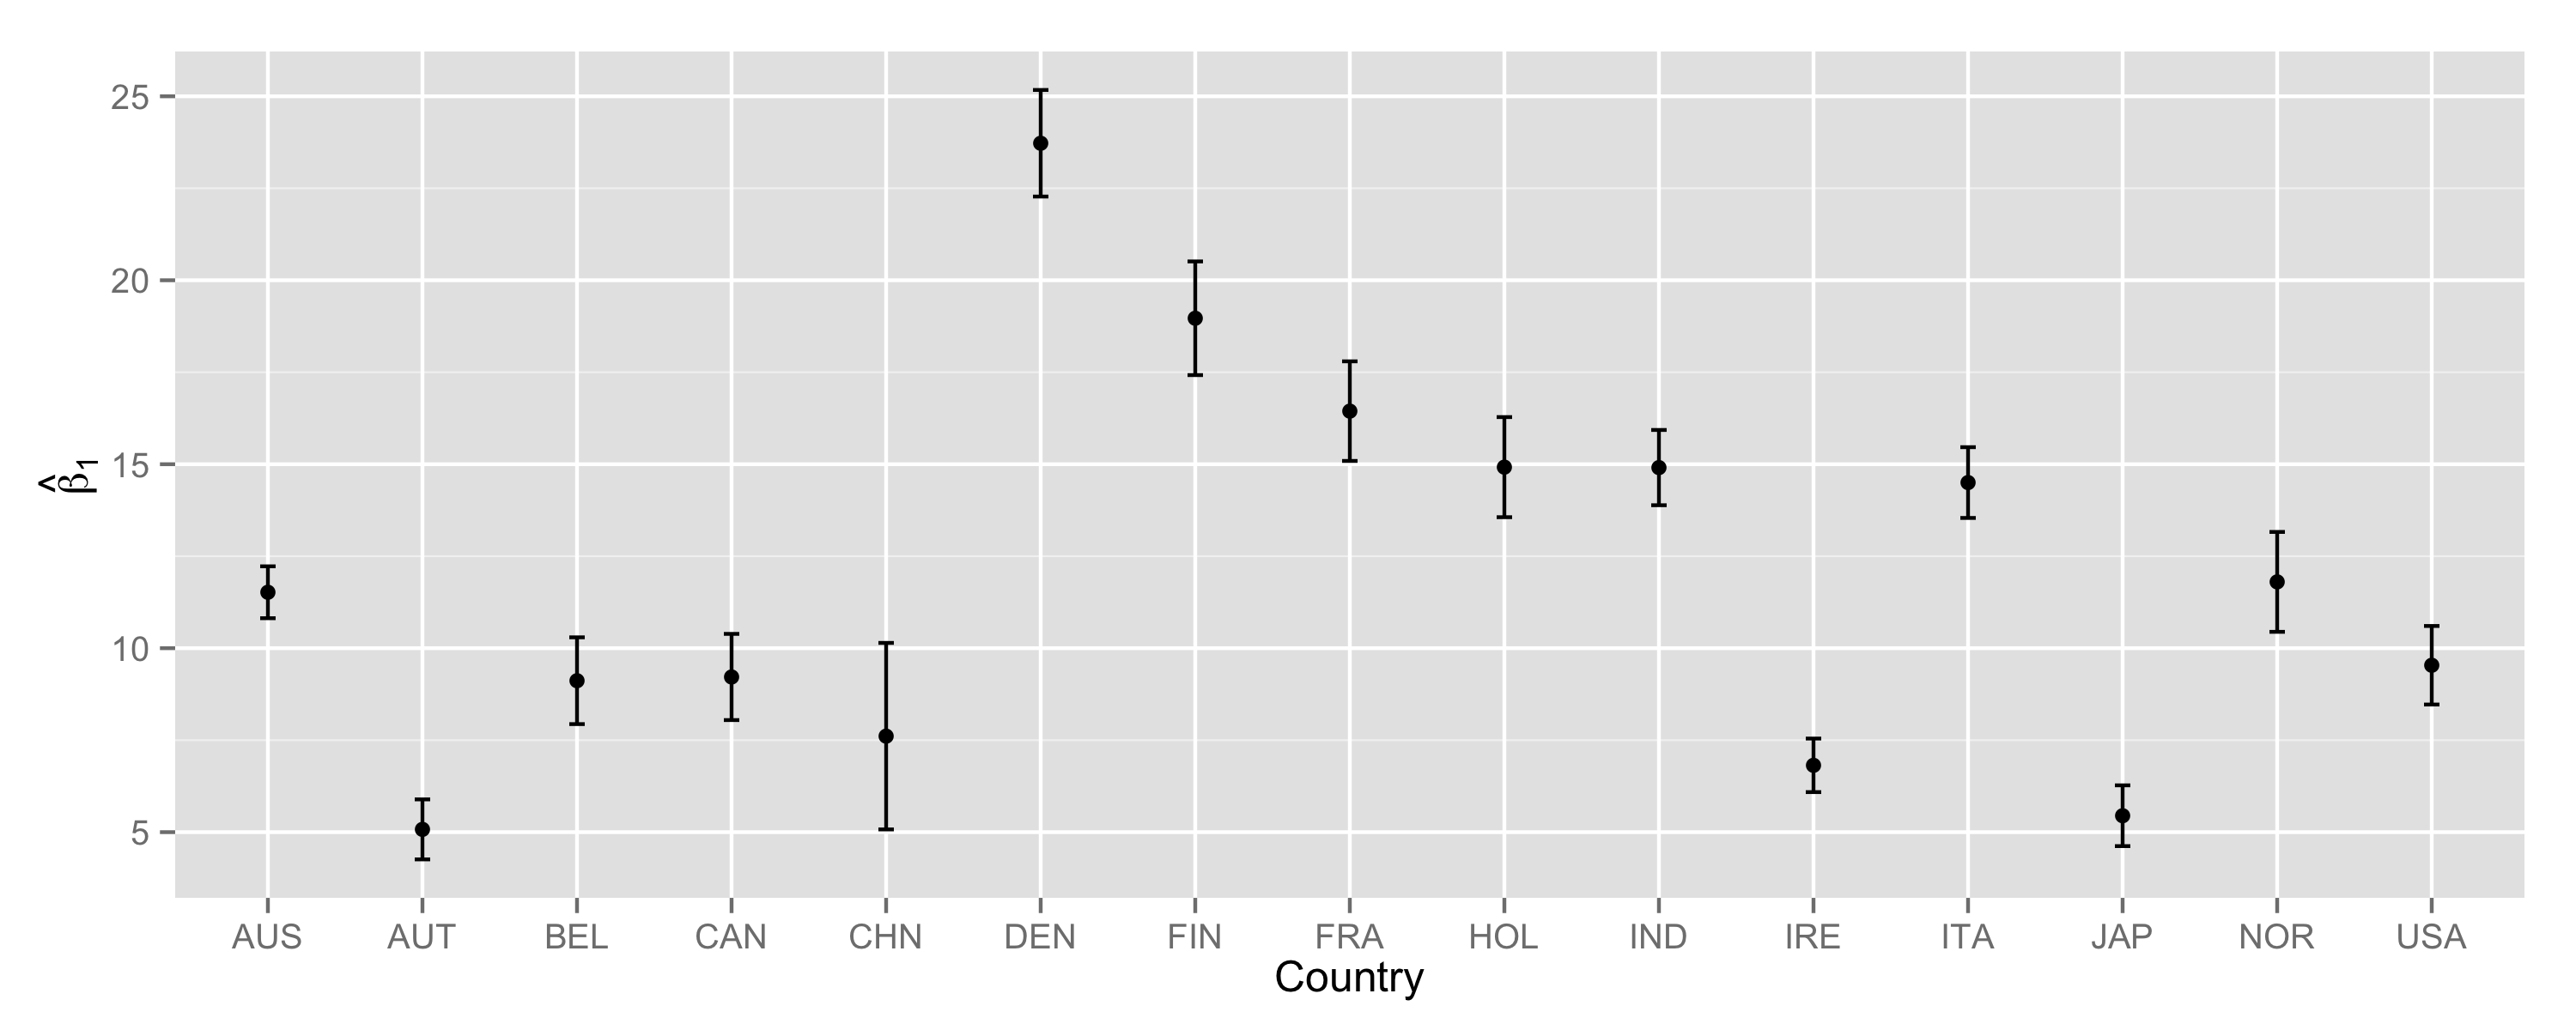
\includegraphics[width=16cm]{b_1_plot} \\
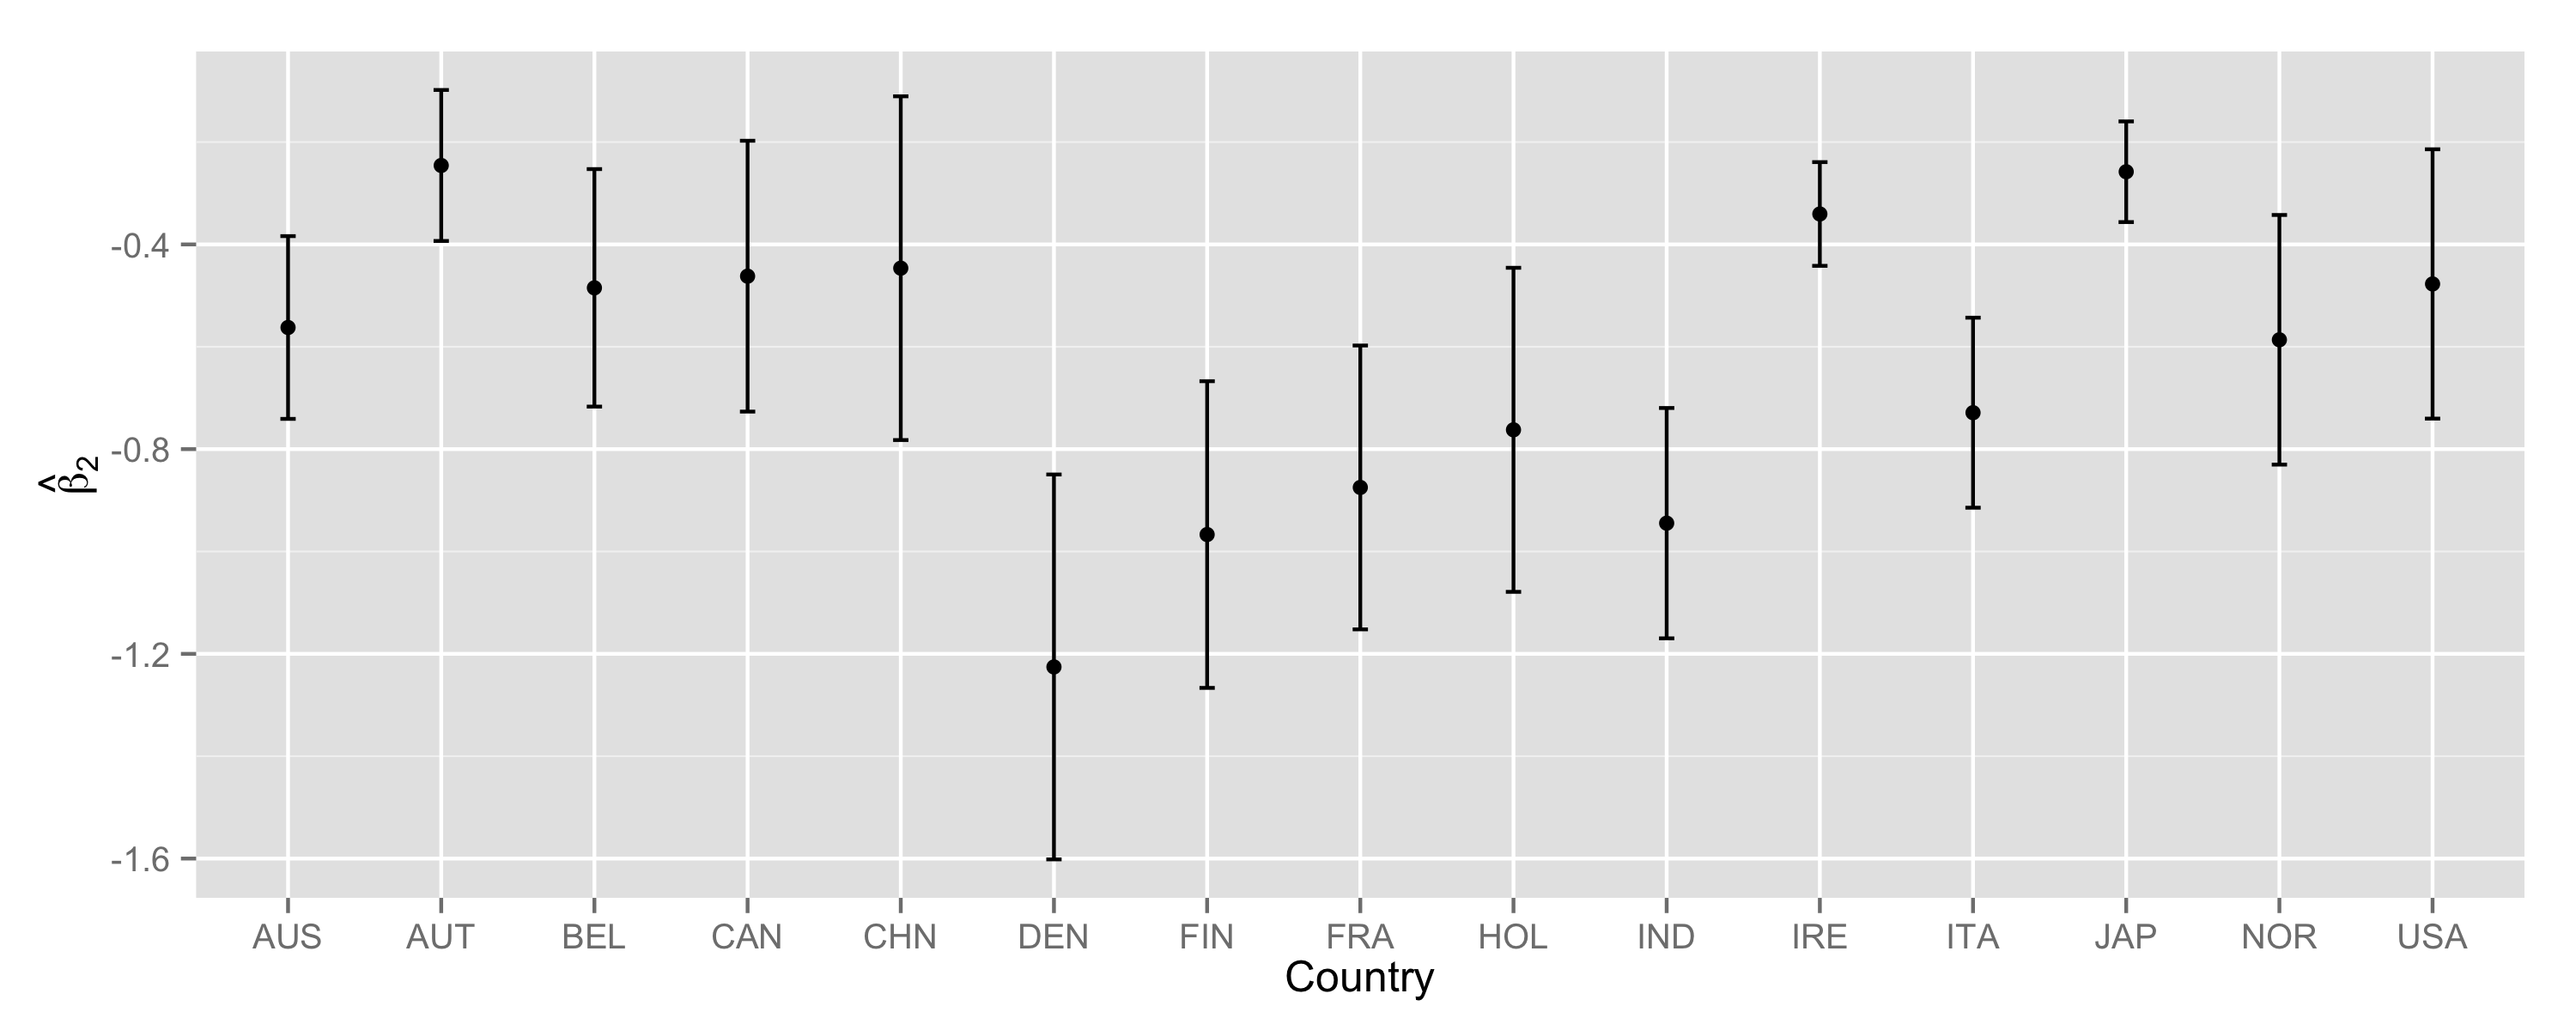
\includegraphics[width=16cm]{b_2_plot} \\
\end{tabular}
}
\end{table}

Table \ref{beta1_est} and \ref{beta2_est} report the estimates and 95\% confidence intervals of parameters $\beta_{1}$ and $\beta_{2}$, and Table \ref{beta12_plot} presents the plots of the results. For the parameter $\beta_{1}$, we can not find any group with more than four groups of countries whose confidence intervals overlap. Such result is consistent with that of \cite{piaggiopadilla2010}. However, for the parameter $\hat{\beta}_{2n}$, among the 15 countries, we can find group of 11 countries whose confidence intervals overlap. Hence, the homogeneity of parameters can not be rejected as in \cite{piaggiopadilla2010}. There are two main reasons for the  differences between our results and theirs. Firstly, they assume the innovation is i.i.d. normally distributed while we allow the error to be serially correlated with itself. Secondly, we incorporate the effect of endogeneity in our limit distribution of estimator. Based on (\ref{example.eqn1}), both reasons will make the critical values and confidence intervals significantly larger than that of \cite{piaggiopadilla2010}.


%%%%%%%%%%%%%%%%%%%%%%%%%%%%%%%%%%%%%%
%                                    %
%                                    %
%            Conclusion              %
%                                    %
%                                    %
%%%%%%%%%%%%%%%%%%%%%%%%%%%%%%%%%%%%%%

\section{Conclusion and discussion} \la{sec:6:conclusion}

In this paper, we establish an asymptotic theory for a nonlinear parametric cointegrating regression model. A general framework is developed for establishing the weak consistency of the NLS estimator $\hat{\theta}_n$. The framework can easily be applied to a wide class of nonstationary regressors, including the partial sum of linear processes and Harris recurrent Markov chains. Limit distribution of $\hat{\theta}_n$ is also established, which  extends previous works. Furthermore, we introduce endogeneity to our model by allowing the error term to be serially dependent on itself, and cross-dependent on the regressor. We show that the limit distribution of $\hat{\theta}_n$ under the endogeneity situation is different from that with martingale error structure. This result is of interest in the applied econometric research area. 

Asymptotics in this paper are limited to univariate regressors and 
nonlinear parametric cointegrating regression models. Specification of the nonlinear regression function $f$ depends usually on the underlying theories of the subject. Illustration can be found in  \cite{baekakkarogaki2004}, where  the concept of the money in the utility function with the constant elasticity of substitution (MUFCES) is used  to relate the money balance with nominal interest rate by the link function $f(x, \al, \beta) = \al + \beta \log(\frac{x}{1 + x})$. More currently, nonparametric method
 has been developed to test the specification of $f$. See, e.g., \cite{wangphillips2012},  for instance.
Extension to multivariate regressors require substantial different techniques. This is because  local time theory can not in general be extended to multivariate data, in which the techniques play a key rule in  the asymptotics of the NLS estimator with nonstationary regressor when $f$ is an integrable function.   Possible extension to multivariate regressors is the index model discussed in \cite{changpark2003}. This again requires some new techniques, and hence we leave it for future  work.


%%%%%%%%%%%%%%%%%%%%%%%%%%%%%%%%%%%%%%
%                                    %
%                                    %
%       Proofs of main results       %
%                                    %
%                                    %
%%%%%%%%%%%%%%%%%%%%%%%%%%%%%%%%%%%%%%

\section{Proofs of main results} \la{sec:6:proof}

This section provides proofs of the main results. We start with some preliminaries, which list the limit theorems that are commonly used in the proofs of the main results.

\subsection{Preliminaries}

Denote $\mathcal N_{\de}(\theta_0) = \{ \theta: \| \theta - \theta_0\| < \de\}$, where $\theta_0 \in \Theta$ is fixed.
\begin{lem} \la{lemClose} Let Assumption \ref{assumpClose} hold. Then, for any $x_t$ satisfying   (\ref {20}) with $T$ being given as in Assumption \ref{assumpClose},
\be \la{lemClose.eqn0}
\sup_{\theta \in \mathcal N_{\de}(\theta_0)} \kappa_n^{-2} \sum_{t = 1}^n \big(|f(x_t, \theta) - f(x_t, \theta_0)| + |f(x_t, \theta) - f(x_t, \theta_0)|^2\big)  &\to_P& 0,
\ee
as $n\to\infty$ first and then $\de \to 0$. If in addition Assumption \ref{assumpMartingale}, then
\be
\kappa_n^{-2} \sum_{t = 1}^n [f(x_t, \theta_0) - f(x_t, \pi_0)]\, u_t   \to_P 0, \la {98}
\ee
for any $\theta_0,\pi_0\in \Theta$, and
\be
\la{lemClose.eqn1}
\sup_{\theta \in \mathcal N_{\de}(\theta_0)}  \kappa_n^{-2} \sum_{t = 1}^n |f(x_t, \theta) - f(x_t, \theta_0)|\, |u_t|  \to_P 0,
\ee
as $n\to\infty$ first and then $\de \to 0$.
\end{lem}

\begin{proof} (\ref {lemClose.eqn0}) is simple.
As $\kappa_n^{-2} \sum_{t = 1}^n [f(x_t, \theta_0) - f(x_t, \pi_0)]^2\le C\kappa_n^{-2} \sum_{t = 1}^n T^2(x_t)=O_P(1)$,
(\ref {98}) follows from Lemma 2 of \cite{laiwei1982}. As for (\ref {lemClose.eqn1}), the result follows from
\bestar
\sum_{t = 1}^n |f(x_t, \theta) - f(x_t, \theta_0)|\, |u_t| \le h(\|\theta-\theta_0\|)\sum_{t = 1}^n T(x_t)\, |u_t|,
\eestar
and $\sum_{t = 1}^n T(x_t)\, |u_t|\le C\sum_{t = 1}^n T(x_t)+
\sum_{t = 1}^n T(x_t)\,\big[ |u_t|-E(|u_t|\mid {\cal F}_{t-1})\big] =O_P(\kappa_n^{2})$.
\end{proof}





\begin{lem} \la{lemJoint} Let Assumption \ref{ad1} (i) hold.
 For any bounded $g (x)$ satisfying  $\int_{-\infty}^{\infty} |g(x)| dx < \infty$, we have
\be
\sum_{t = 1}^n g(x_t) &=& O_P(n/d_n). \la {tya}
\ee
If in addition Assumption \ref{ad1} (ii)--(iii), then, for any bounded $g_i(x), i=1,2,$
satisfying $\int_{-\infty}^{\infty} |g_i(x)| dx < \infty$ and $\int_{-\infty}^{\infty} g_i(x) dx  \ne 0$,
\be \la{lemJoint.eqn1}
\Big \{ \big(\frac {d_n}n\big)^{1/2}\sum_{t=1}^n g_1(x_t) u_t ,\, \frac {d_n}n\sum_{t=1}^n g_2(x_t) \Big \} &\rightarrow_D& \Big \{\tau_1 \, N \, L^{1/2}_{G}(1,0), \tau_2\, L_{G}(1,0) \Big \},
\ee
 where $\tau_1^2 = \int_{-\infty}^{\infty} g_1^2(s) ds$, $\tau_2= \int_{-\infty}^{\infty} g_2(s) ds$ and $N$ is a standard normal variate independent of $G(t)$.
\end{lem}

\begin{proof} For (\ref {tya}),  see Lemma 3.2 of \cite{wangphillips2009}.
Theorem 2.2 of \cite{wang2011} provides  (\ref {lemJoint.eqn1}) with $g_2(x)=g_1^2(x)$. It is not difficult to see that (\ref {lemJoint.eqn1}) still holds for general $g_2(x)$. We omit the details.
\end{proof}



\begin{lem} \la{lemMarkov} Let Assumption \ref {ad1}*(i) hold. For any $g$ such that $\int_{-\infty}^{\infty} |g(x)| \pi(dx) < \infty$ and $\int_{-\infty}^{\infty} g(x) \pi(dx) \ne 0$, we have
\be
\sum_{t = 1}^n g(x_t) &=& O_P[a(n)], \quad
\big [\sum_{t = 1}^n g(x_t)\big ]^{-1} = O_P[a(n)^{-1}]. \la {ty}
\ee
If in addition Assumption \ref{ad1}* (ii)--(iii), then, for any bounded $g_i(x), i=1,2,$ satisfying $\int_{-\infty}^{\infty} |g_i(x)| \pi(dx) < \infty$ and $\int_{-\infty}^{\infty} g_i(x) \pi(dx)  \ne 0$,
\be \la{lemMarkov.eqn2}
\Big \{ a(n)^{-1/2}\sum_{t=1}^n g_1(x_t) u_t ,\, a(n)^{-1}\sum_{t=1}^n g_2(x_t) \Big \}  \rightarrow_D   \Big \{\tau_5 \, N \, \Pi^{1/2}_{\beta}, \tau_6\,\Pi_\beta \Big \},
\ee
 where $\tau_5^2 = \int_{-\infty}^{\infty} g_1^2(s) \pi(ds)$, $\tau_6= \int_{-\infty}^{\infty} g_2(s) \pi(ds)$, $\Pi_{\beta}$ is defined as in Theorem \ref {thmIntegrablelimit1} and $N$ is a standard normal variate independent of $\Pi_\beta$.
\end{lem}


\begin{proof}
The proof of (\ref {ty}) sees Theorem 2.1 of \cite{chen1999}. To prove (\ref{lemMarkov.eqn2}), we first impose an additional assumption that $g_2(x) = g_1^2(x)$. Denote
\be
\Delta^2_n = a(n)^{-1}\sum_{t = 1}^n g_1^2(x_t), \quad Z_{nt} = a(n)^{-1/2}g_1(x_t) \Delta_n^{-1}, \quad  \mbox{and} \quad W_n = \sum_{t = 1}^n Z_{nt} u_k.
\ee
Recalling that $E(u_t|\F_{nt}) = 0$, it is readily seen that given $\{x_1, ..., x_n\}$, $\{Z_{nt} u_t, \F_{nt}\}_{t = 1}^n$ forms a martingale difference sequence. The result (\ref{lemMarkov.eqn2}) will follow if we prove,
\be \la{prfMarkov.eqn1}
\sup_{x} \big | P\big ( W_n \le x \, | \, x_1, ..., x_n \big ) - \Phi(x) \big | \to_P 0.
\ee
%\begin{align}
%\sum_{t = 1}^n |Z_{nt}|^q &\to_P 0, \\
%\sum_{t = 1}^{\tau_n(t)} Z_{nt}^2 \,E(u_t^2 | \F_{nt}) &\to_P t,
%\end{align}
%for all $t \in [0, 1]$.

\noindent Indeed, by noting that $\Delta_n^2$ is measurable with respect to $\si(x_1,...x_n)$, we have, for any $\al, \gamma \in R$,
\begin{align}
&\big |E \big [ e^{i  \al  W_n + i \beta \Delta_n^2} \big ] - e^{-\frac{1}{2} \al^2 } \, E\big [e^{i \beta \tau_5 \Pi_\gamma} \big ] \big| \no\\
&\le E \Big |E \big ( e^{i \al W_n } |\, x_1, ..., x_n \big ) - e^{-\frac{1}{2}\al^2 } \,  \Big| +e^{-\frac{1}{2}\al^2}\Big| Ee^{i \gamma \Delta_n^2} - Ee^{i \gamma \tau_5 \Pi_\beta} \Big | \to 0, \no
\end{align}
by dominated convergence theorem, due to (\ref{prfMarkov.eqn1}) and $\Delta_n^2 \to_D \tau_5 \Pi_\beta$ (see, e.g., Theorem 2.3 of \cite{chen1999}). This implies that
\bestar
\{ W_n, \Delta_n^2 \} \to_D \{N, \tau_5\Pi_\beta\},
\eestar
where $N$ is a standard normal random variable independent of $\Pi_\beta$. Hence, by continuous mapping theorem, we have
\bestar
\Big \{ a(n)^{-1/2}\sum_{t=1}^n g_1(x_t) u_t ,\, a(n)^{-1}\sum_{t=1}^n g_1^2(x_t) \Big \} = \Big \{ \Delta_n W_n, \Delta_n^2\Big \}\to_D \{\tau_5^{1/2} N\Pi_\beta^{1/2}, \tau_5\Pi_\beta\},
\eestar
which implies the required (\ref{lemMarkov.eqn2}).

We now prove (\ref{prfMarkov.eqn1}). By Theorem 3.9 ((3.75) there) in \cite{hallheyde1980} with $\de = q/2 - 1$ that
\bestar
\sup_{x} \big | P\big ( W_n \le x \, | \, x_1, ..., x_n \big ) - \Phi(x) \big | \le A(\de) \mathcal L_n^{1 / (1 + q)}  \quad a.s.,
\eestar
where $A(\de)$ is a constant depending only on $\de$ and $q > 2$, and (set $\F^*_n = \si(x_1, ..., x_n)$)
\bestar
\mathcal L_n = \Delta_n^{-q} \sum_{k = 1}^n |Z_{nk}|^q E(|u_k|^q | \F^*_{n}) + E \Big [ \big | \Delta_n^{-2} \sum_{k = 1}^n Z_{nk}^2 [E(u_k^2 | \F_{nk}) - 1] \big|^{q/2} \Big | \, \F^*_{n} \Big].
\eestar
Recall from Assumption \ref{ad2} (iv) and the fact that $\Delta_n^2 = \sum_{k = 1}^n Z^2_{nk}$, we have,
\bestar
E \Big [ \big | \Delta_n^{-2} \sum_{k = 1}^n Z_{nk}^2 [E(u_k^2 | \F_{nk}) - 1] \big|^{q/2} \Big | \, \F^*_{n} \Big] \to_P 0,
\eestar
by dominated convergence theorem. Hence,  routine calculations show that
\bestar
\mathcal L_n \le C\,\Delta_n^{-(q-2)} \,a(n)^{-(q-2)/2} + o_P(1) = o_P(1),
\eestar
because $\Delta_n^{-2}=O_P(1)$ by (\ref{ty}) and $q > 2$. This proves (\ref{prfMarkov.eqn1}), which implies that (\ref{lemMarkov.eqn2}) holds true with $g_2(x) = g_1^2(x)$. Finally, note that, for any $a$, $b \in R$,
\bestar
a(n)^{-1} \sum_{t = 1}^n \big \{ a g_1^2(x_t) + bg_2(x_t)\big  \}  \to_D  \int_{-\infty}^{\infty} \big [a g_1^2(s) + bg_2(s) \big ] \pi(ds)\, \Pi_\beta,
\eestar
due to Theorem 2.3 of \cite{chen1999}, which implies that
\bestar
\Big \{ a(n)^{-1}\sum_{t=1}^n g_1^2(x_t) ,\, a(n)^{-1}\sum_{t=1}^n g_2(x_t) \Big \}\to_D  \Big \{\int_{-\infty}^{\infty} g_1^2(s) \pi(ds)\, \Pi_\beta, \int_{-\infty}^{\infty} g_2(s) \pi(ds)\, \Pi_\beta, \Big \}.
\eestar
Hence, by continuous mapping theorem,
\bestar
\frac{ \sum_{t=1}^n g_1^2(x_t) }{\sum_{t=1}^n g_2(x_t)} \to_P \int_{-\infty}^{\infty} g_1^2(s)\,  \pi(ds) \Big /  \int_{-\infty}^{\infty} g_2(s) \, \pi(ds) .
\eestar
This shows that (\ref{lemMarkov.eqn2}) is still true with general $g_2(x)$.
\end{proof}


\begin{lem} \la{lemLagJoint} Under Assumption \ref {4.1}, for any bounded $g_i(x), i=1,2,$
satisfying $\int_{-\infty}^{\infty} |g_i(x)|dx < \infty$ and $\int_{-\infty}^{\infty} g_i(x) dx  \ne 0$, we have
\be \la{lemLagJoint.eqn1}
 \sum_{t = 1}^n g_1(x_t) |u_t| = O_P(n / d_n),
\ee
and
\be \la{lemLagJoint.eqn2}
&\Big \{ (n/d_n)^{-1/2}\sum_{t=1}^n g_1(x_t) u_t ,\, (n/d_n)^{-1}\sum_{t=1}^n g_2(x_t) \Big \} \no\\
&\quad \rightarrow_D \Big \{\tau_3 \, N \, L^{1/2}_{G}(1,0), \tau_4 L_{G}(1,0) \Big \},
\ee
 where $\tau_3^2 = (2\pi)^{-1}\int_{-\infty}^{\infty}\hat{g}_1(\mu)^2 [ Eu_0^2 + 2 \sum_{r = 1}^{\infty}E(u_0u_r e^{-i\mu x_r})]\,d\mu$, $\hat{g}_1(\mu)=\int_{-\infty}^{\infty}e^{i\mu x}g_1(x) dx$ and $\tau_4 = \int_{-\infty}^{\infty} g_2(s) ds$.
\end{lem}

\begin{proof}
See Theorem 3 and 5 of \cite{jaganathan2008}.
\end{proof}

\begin{lem} \la{lemEndo} Under Assumption \ref{4.2}, for any twice continuous differentiable function $g_i(x)$, $i = 1, 2$, satisfying $|g_i'(x)| \le K (1 + |x|^{\al})$ for some constants $K, \al > 0$ for all $x \in R$, and if $q \ge \max(3, 2\al)$ where $q$ is given Assumption \ref{4.2}, we have
\begin{align} \la{lemEndo.eqn1}
&\Big \{ \frac{1}{\sqrt{n}} \sum_{t = 1}^{n} g_1 \Big ( \frac{x_t}{\sqrt{n}}\Big) u_t, \frac{1}{n} \sum_{t = 1}^{n} g_2  \Big ( \frac{x_t}{\sqrt{n}}\Big) \Big \} \no\\
&\to_D \Big \{ \sigma_{\xi u} \int_{0}^{1} g_1'(W(t))dt + \int_0^1 g_1(W(t)) dU(t), \int_0^1 g_2(W(t)) dt\Big \},
\end{align}
as $n \to \infty$, where $\si_{\xi u} = \sum_{j = 0}^{\infty} E( \xi_0 u_j)$, and $(W(t), U(t))$ is a bivariate Brownian motion with covariance matrix
\bestar
\Delta = \begin{pmatrix}
\phi^2 E\ep_0^2 & \phi \psi E \ep_0 \nu_0 \\
\phi\psi E \ep_0 \nu_0 & \psi^2 E\nu_0^2
\end{pmatrix}.
\eestar
\end{lem}
\begin{proof} See Theorem 4.3 of \cite{ibragimovphillips2008} with minor improvements.
We omit the details.
\end{proof}

\begin{lem} \la{lemC}
Under Assumptions \ref{ad1}(i) and  \ref {ad2},   we have
\be \la{lemC.eqn1}
\frac {d_n}n\,\sup_{\theta \in \mathcal N_{\de}(\theta_0)}
\sum_{t = 1}^n \big|\dot f_i(x_t, \theta)\,\dot f_j(x_t, \theta) - \dot f_i(x_t, \theta_0)\,\dot f_j(x_t, \theta_0)\big|  &\to_P& 0, \\
\frac {d_n}n\,\sup_{\theta \in \mathcal N_{\de}(\theta_0)}\la{lemC.eqn2}
\sum_{t = 1}^n \big|\ddot f_{ij}(x_t, \theta)\,[ f(x_t, \theta) -  f(x_t, \theta_0)]\big|  &\to_P& 0,
\ee
as $n\to\infty$ first and then $\de \to 0$,  for any $1\le i, j\le m$. If in addition Assumption \ref{ad1} (ii)--(iii), then
\be\la{lemC.eqn3}
\frac {d_n}n\,\sup_{\theta \in \mathcal N_{\de}(\theta_0)}\big| \sum_{t = 1}^n\ddot f_{ij}(x_t, \theta)\,u_t \big| \to_P 0,
\ee
as $n\to\infty$ first and then $\de \to 0$,  for any $1\le i, j\le m$.

Similarly, under Assumptions \ref{ad1}* (i) and  \ref {ad2}*,
(\ref {lemC.eqn1}) and (\ref {lemC.eqn2}) are  true if we replace $d_n / n$ by $a(n)^{-1}$. If in addition Assumption \ref{ad1}* (ii) and (iii), then (\ref {lemC.eqn3})
 holds if we replace $d_n / n$ by $a(n)^{-1}$.
\end{lem}


\begin{proof} We only prove (\ref{lemC.eqn1}). Others are similar and the details are omitted. First note that, by Assumption \ref{ad2} (i) and (iii),
\begin{align}
\sup_{\theta \in \Theta} |f_i(x_t, \theta)| &\le \sup_{\theta \in \Theta} |\dot{f}_i(x_t, \theta)-\dot{f}_i(x_t, \theta_0)| + |\dot{f}_i(x_t, \theta_0)| \no\\
 &\le \sup_{\theta \in \Theta} h(\| \theta - \theta_0\|)T(x_t) + |\dot{f}_i(x_t, \theta_0)| \le C. \no
\end{align}
It follows that
\bestar
&& \big|\dot f_i(x_t, \theta)\,\dot f_j(x_t, \theta) - \dot f_i(x_t, \theta_0)\,\dot f_j(x_t, \theta_0)\big| \no\\
&\le& \big|\dot f_i(x_t, \theta) \big |\big|\dot f_j(x_t, \theta)- \dot f_j(x_t, \theta_0)\big| + \big|\dot f_j(x_t, \theta_0) \big |\big|\dot f_i(x_t, \theta) - \dot f_i(x_t, \theta_0)\big| \no\\
&\le& C\big|\dot f_j(x_t, \theta)- \dot f_j(x_t, \theta_0)\big| +C_1\big|\dot f_i(x_t, \theta) - \dot f_i(x_t, \theta_0)\big|.
\eestar
Therefore, by recalling (\ref {tya}), the result (\ref{lemC.eqn1}) follows
from an application of Lemma \ref{lemClose} with $\kappa_n^2=n/d_n$.
\end{proof}

\begin{lem}  \la{lemHomoC}
 Under Assumptions \ref{assumpLimitHomo1} and \ref{assumpLimitHomo2},   we have
\be \la{lemC.eqn1a}
\frac {1}{n\dot v_i (d_n)\dot v_j (d_n)}\,\sup_{\theta \in \mathcal N_{\de}(\theta_0)}
\sum_{t = 1}^n \big|\dot f_i(x_t, \theta)\,\dot f_j(x_t, \theta) - \dot f_i(x_t, \theta_0)\,\dot f_j(x_t, \theta_0)\big|  &\to_P& 0, \\
\frac {1}{nv(d_n)\ddot v_{ij} (d_n)}\,\sup_{\theta \in \mathcal N_{\de}(\theta_0)}\la{lemC.eqn2a}
\sum_{t = 1}^n \big|\ddot f_{ij}(x_t, \theta)\,[ f(x_t, \theta) -  f(x_t, \theta_0)]\big|  &\to_P& 0,\\
\la{lemC.eqn3a}
\frac {1}{n\ddot v_{ij} (d_n)}\,\sup_{\theta \in \mathcal N_{\de}(\theta_0)}\big| \sum_{t = 1}^n\ddot f_{ij}(x_t, \theta)\,u_t \big| &\to_P& 0,
\ee
as $n\to\infty$ first and then $\de \to 0$,  for any $1\le i, j\le m$.
\end{lem}

\begin{proof}  Recall $\max_{1\le t\le n}|x_t|/d_n=O_P(1)$. Without loss of generality, we assume $\max_{1\le t\le n}|x_t|/d_n\le K_0$ for some $K_0>0$.
It follows from Assumption \ref {assumpLimitHomo2} and $d_n \to \infty$  that, for any $1\le i\le m$ and $\theta\in \Theta$,
\bestar
\big|\dot f_i(x_t, \theta)\big| &\le& \dot v_i (d_n)\big( |\dot h_i(x_t/d_n)|+o(1)\, T_{1\dot f_i}(x_t/d_n) \big),\\
\big|\dot f_i(x_t, \theta) - \dot f_i(x_t, \theta_0)\big| &\le& A_{\dot f_i}(||\theta-\theta_0||)\dot v_i (d_n) T_{1\dot f_i}(x_t/d_n).
\eestar
This implies that
\be
&& \sup_{\theta \in \mathcal N_{\de}(\theta_0)}
\sum_{t = 1}^n \big|\dot f_i(x_t, \theta)\,\dot f_j(x_t, \theta) - \dot f_i(x_t, \theta_0)\,\dot f_j(x_t, \theta_0)\big| \no\\
&\le&2\, (A_{\dot f_i}(\delta)+A_{\dot f_j}(\delta))\, \dot v_i (d_n)\dot v_j (d_n)\, \sum_{t = 1}^n\big( |\dot h_i(x_t/d_n)|+ T_{1\dot f_i}(x_t/d_n) \big).\la{lemHomoC.eqn1}
\ee
(\ref {lemC.eqn1a}) now follows from $A_{\dot f_i}(\delta)\to 0$ as $\delta\to 0$ and
\bestar
\frac 1n\sum_{t = 1}^n\big[ |\dot h_i(x_t/d_n)|+ T_{1\dot f_i}(x_t/d_n) \big]\to_D \int_0^1\big[ |\dot h_i(G(t))|+ T_{1\dot f_i}(G(t))\big] dt=O_P(1),
\eestar
due to Assumptions \ref{assumpLimitHomo1} (iii) and 3.4 (iii).

The proof of (\ref {lemC.eqn2a}) is similar and hence the details are omitted. As for (\ref {lemC.eqn3a}), by noting
\bestar
\big| \sum_{t = 1}^n\ddot f_{ij}(x_t, \theta)\,u_t \big|\le \big| \sum_{t = 1}^n\ddot f_{ij}(x_t, \theta_0)\,u_t \big|+ \sum_{t = 1}^n|\ddot f_{ij}(x_t, \theta)-\ddot f_{ij}(x_t, \theta_0)|\,|u_t|,
\eestar
the result can be proved by using the similar arguments as in (\ref {98}) and (\ref {lemClose.eqn1}) of Lemma \ref {lemClose}.
\end{proof}

\begin{lem} \la{lemad}  Let Assumption \ref{assumpLimitHomo1} hold. Then, for any regular functions $g(x, \theta)$ and $g_1(x, \theta)$ on $\Theta$, we have
\be
&& \Big\{\frac 1{\sqrt n}\sum_{t=1}^ng\Big (\frac {x_t}{d_n}, \theta\Big )\, u_t,\ \frac 1{ n}\sum_{t=1}^ng_1\Big (\frac {x_t}{d_n}, \theta\Big)\Big\} \no\\
&&\qquad \to_D\ \Big\{\int_0^1 g\big(G(t), \theta\big)dU(t),\ \int_0^1 g_1\big(G(t), \theta\big)dt\Big\}.
\ee
\end{lem}

\begin{proof} If $g(x, \theta)$ and $g_1(x, \theta)$ are continuous functions, the result follows from (\ref {nm1}) and the continuous mapping theorem. See, \cite{kurtzprotter1991} for instance. The extension from continuous function to regular function is standard in literature. The details can be found in PP or \cite{parkphillips1999}.
\end{proof}

\begin{lem} \la{lemWu} Let $D_n(\theta, \theta_0) =  Q_n(\theta) - Q_n(\theta_0)$.
 Suppose that, for any $\de > 0$,
\be \la{lemWu.eqn1}
\liminf_{n \to \infty} \inf_{|\theta - \theta_0| \ge \delta} D_n(\theta, \theta_0) > 0 \quad in \quad  probability,
\ee
 then $\hat{\theta}_n \rightarrow_P \theta_0$.
\end{lem}

\begin{proof}
See Lemma 1 of \cite{wu1981}.
\end{proof}



\subsection{Proof of Theorems}

\begin{proof}[Proof of Theorem \ref {thmConsistency}]
Let $\mathcal N$ be any open subset of $\Theta$ containing $\theta_0$. Since $\hat{\theta}_n$ is the minimizer of $Q_n(\theta)$ over $\theta \in \Theta$,  by Lemma \ref{lemWu}, proving consistency is equivalent to showing that, for any $0<\eta<1$ and $\theta \ne \theta_0$, where $\theta, \theta_0\in \Theta$, there exist
 $n_0 > 0$ and $M_1>0$ such that
\be \la{prfConsistency.eqn1}
P \Big ( \inf_{\theta \in \Theta \cap \mathcal N^c}\, D_n(\theta, \theta_0) \ge  \kappa^2_n /M_1 \Big ) \ge 1 - \eta,
\ee
for all $n > n_0$.

Denote $\mathcal N_{\de}(\pi_0) = \{ \theta: \| \theta - \pi_0\| < \de\}$. Note that $\Theta \cap \mathcal N^c$ is compact, by the finite covering property of compact set, (\ref{prfConsistency.eqn1}) will follow if we prove that, for any fixed $\pi_0 \in \Theta \cap \mathcal N^c$,
\be \la{prfConsistency.eqn2}
\sup_{\theta \in \mathcal N_{\de}(\pi_0)} \kappa_n^{-2} \Big | D_n(\theta, \theta_0) - D_n(\pi_0, \theta_0) \Big | \to_P 0,
\ee
as $n\to\infty$ first and then $\de \to 0$, and for $\forall \ep>0$, there exists $M_1 > 0$ and $n > n_0$ such that for all $n > n_0$,
\be \la{prfConsistency.eqn3}
P\Big ( D_n(\pi_0, \theta_0) \ge \kappa^2_n/M_1 \Big ) \ge 1 -2 \eta.
\ee
The result  (\ref{prfConsistency.eqn2}) is simple. Indeed, by Lemma \ref{lemClose},  for each fixed $\pi_0 \in \Theta \cap \mathcal N^c$, we have
\begin{align}
&\sup_{\theta \in \mathcal N_{\de}(\pi_0)}\kappa_n^{-2}\Big | D_n(\theta, \theta_0) - D_n(\pi_0, \theta_0) \Big | \no\\
&\le \sup_{\theta \in \mathcal N_{\de}(\pi_0)} \kappa_n^{-2}\sum_{t=1}^n (f(x_t, \theta) - f(x_t, \pi_0))^2 \no\\
&\hskip 3.5cm + \sup_{\theta \in \mathcal N_{\de}(\pi_0)}\kappa_n^{-2} \sum_{t = 1}^n |f(x_t, \theta) - f(x_t, \pi_0)|| u_t|\no\\
&\to_P 0,
\end{align}
as $n\to\infty$ first and then $\de \to 0$, which yields (\ref {prfConsistency.eqn2}).

To prove (\ref{prfConsistency.eqn3}), we  recall
\bestar
D_n(\pi_0, \theta_0) =  \sum_{t = 1}^n (f(x_t, \pi_0) - f(x_t, \theta_0))^2 -  \sum_{t = 1}^n (f(x_t, \pi_0) - f(x_t, \theta_0)) u_t.
\eestar
This, together with (\ref {21}) and (\ref {98}), implies that,
 for any $\eta>0$, there exists $n_0 > 0$ and $M_1 > 0$ such that for all $n > n_0$,
\begin{align}
P\Big ( D_n(\pi_0, \theta_0) \ge \kappa^2_n M_1^{-1} \Big ) &\ge P \Big ( \sum_{t = 1}^n ( f(x_t, \pi_0) - f(x_t, \theta_0))^2 \ge \kappa^2_n\, M_1^{-1}/2 \Big ) - \eta \no\\
&\ge1 -2 \eta, \no
\end{align}
which implies (\ref{prfConsistency.eqn3}).

Finally, by noting $Q_n(\theta_0) = n^{-1} \sum_{t = 1}^n u_t^2 \to_P \si^2$ due to  Assumption \ref{assumpMartingale} and strong law of large number,  it  follows from the consistency of $\hat{\theta}_n$ and (\ref{prfConsistency.eqn2}) that
\bestar
|\hat{\si}_n^2 - \si^2| \le C \kappa_n^{-2} |Q_n(\hat{\theta}_n) - Q_n(\theta_0)| + o_P(1) = o_P(1).
\eestar
\end{proof}


\begin{proof}[Proof of Theorem \ref {thmLinearConsistency}]
(\ref {20}) follows from (\ref {tya}) of Lemma \ref{lemJoint}.
(\ref {21}) follows from (\ref {lemJoint.eqn1}) of Lemma \ref{lemJoint} with $g_2(x)=(f(x, \theta)-f(x, \theta_0))^2$ and the facts that $P(L_G(1,0) > 0) = 1$ and $\int_{-\infty}^{\infty} (f(s, \theta) - f(s, \theta_0))^2 ds > 0$, for any $\theta \ne \theta_0$.
\end{proof}


\begin{proof}[Proof of Theorem \ref {thmMarkovConsistency}]
 (\ref {20}) follows from (\ref {ty}) of  Lemma \ref{lemMarkov} with $g(x)=T(x)+T^2(x)$.
  (\ref {21}) follows from (\ref {lemMarkov.eqn2}) of Lemma \ref{lemMarkov} with   $g_2(x)=(f(x, \theta)-f(x, \theta_0))^2$ and the facts that
   $P(\Pi_{\beta}> 0) = 1$ and $\int_{-\infty}^{\infty} (f(s, \theta) - f(s, \theta_0))^2 \pi(ds) > 0$, for any $\theta \ne \theta_0$.
\end{proof}

\begin{proof}[Proof of Theorem \ref {thmHomoConsistency}]
Recalling $T(\lam x)\le v(\lam)\, T_1(x)$,  we have
\be
\frac{1}{nv^2(d_n)} \sum_{t = 1}^n [T(x_t) + T^2(x_t)] &\le& \frac{1}{n} \sum_{t = 1}^n \big [T_1\Big (\frac{x_{t}}{ d_n}  \Big) + T_1^2\Big (\frac{x_{t} }{d_n}  \Big) \big ]\no\\
&\to_D&\int_0^1[T_1(G(t))+T_1^2(G(t))]dt, \la {101}
\ee
where the convergence in distribution comes from \cite{berkeshorvath2006}.
This proves (4) with $\kappa_n = \sqrt{n}v(d_n) $ due to the local integrability of $T_1+T_1^2$.
To prove (5), by letting $G(\lambda, x) := f(\lambda x, \theta) - f(\lambda x, \theta_0) - v(\lambda) g(x,\theta, \theta_0)$, we have
\begin{align}
&\frac{1}{nv^2(d_n)} \sum_{t = 1}^n ( f(x_t, \theta) - f(x_t, \theta_0))^2  \no\\
&=\frac{1}{nv^2(d_n)} \sum_{t = 1}^n \Big [G\Big (d_n, \frac{x_t}{d_n} \Big ) + v(d_n) g\Big(\frac{x_t}{d_n},\theta, \theta_0\Big)\Big]^2  \no\\
&\ge  \frac{1}{n} \sum_{t = 1}^n g^2\Big(\frac{x_t}{d_n},\theta, \theta_0\Big) - | \Lambda_n |,   \la{prf.HomoConsistency.eqn0}
\end{align}
where $\Lambda_n =  \frac{2}{nv(d_n)}\sum_{t = 1}^n   G\Big (d_n, \frac{x_t}{d_n} \Big ) \,g\Big(\frac{x_t}{d_n},\theta, \theta_0\Big)$.
The similar arguments as in the proof of (\ref {101}) yield that
\be
\frac{1}{n} \sum_{t = 1}^n g^2\Big(\frac{x_t}{d_n},\theta, \theta_0\Big) &\to_D& Z:=\int_0^1g^2(G(s), \theta, \theta_0)ds, \la {102}
\ee
where  $P(0<Z<\infty)=1$ due to  Assumption \ref{assumpClose}* (i). On the other hand, it follows from (10) that
\bestar
\frac{1}{nv^2(d_n)}\sum_{t = 1}^n   G^2\Big (d_n, \frac{x_t}{d_n} \Big ) &\le& \frac {o(1)}{nv^2(d_n)}\sum_{t = 1}^n T^2(x_t) \le \frac {o(1)}{n}\sum_{t = 1}^n T_1^2(x_t/d_n) =o_P(1).
\eestar
Now (5) follows from (\ref{prf.HomoConsistency.eqn0}), (\ref {102}) and the fact that
\bestar
\Lambda_n
 \le 2\Big |  \frac{1}{nv^2(d_n)}\sum_{t = 1}^n   G^2\Big (d_n, \frac{x_t}{d_n} \Big )\Big |^{1/2}\,  \Big |\frac{1}{n}\sum_{t = 1}^n \,g^2\Big(\frac{x_t}{d_n},\theta, \theta_0\Big)  \Big |^{1/2} \to_P 0.
\eestar
\end{proof}


\begin{proof}[Proof of Theorem \ref {thmHomoConsistent1}] Let $\Theta_0 = \{ \| \theta - \theta_0 \| \ge \de \}$ where  $\de>0$ is a constant.
By virtue of Lemma \ref{lemWu},   it suffices to prove that, for any $\eta, M_0 >0$, there exist a $n_0 >0$ such that, for all $n > n_0$,
\be \la{prfHomoConsistent2.eqn1}
P \Big (n^{-1} \inf_{\theta \in \Theta_0} D_n(\theta, \theta_0) > M_0 \Big ) > 1-  \eta.
\ee
To prove (\ref{prfHomoConsistent2.eqn1}),  first note that  $\sum_{t=1}^nu_t^2/n\le M_0$ in probability, for some $M_0>0$, due to the Assumption 2.2 (i). This, together with Cauchy-Schwarz Inequality, yields that
\begin{align}
&n^{-1}D_n(\theta, \theta_0) \no\\
& \quad = \frac{1}{n} \sum_{t = 1}^n (f(x_t, \theta) - f(x_t, \theta_0))^2 - \frac{2}{n} \sum_{t = 1}^n (f(x_t, \theta) - f(x_t, \theta_0))u_t  \no\\
&\quad \ge \frac{1}{n} \sum_{t = 1}^n (f(x_t, \theta) - f(x_t, \theta_0))^2 - \frac{2}{n}\Big ( \sum_{t = 1}^n (f(x_t, \theta) - f(x_t, \theta_0))^2 \Big )^{1/2} \Big (\sum_{t = 1}^n u^2_t \Big )^{1/2}  \no\\
&\quad \ge M_n(\theta, \theta_0)\Big [1  - \frac{2\sqrt{M_0 + o_P(1) }}{M_n(\theta, \theta_0 )^{1/2} } \Big ] ,
\end{align}
where $M_n(\theta, \theta_0)=
 \frac{1}{n} \sum_{t = 1}^n (f(x_t, \theta) - f(x_t, \theta_0))^2$. Hence, for any equivalent process $x_{k}^*$ of $x_k$ (i.e., $x_{k}^*=_D x_{k}, 1\le
k\le n, n\ge 1$, where $=_D$ denotes equivalence in distribution), we have
\be
P \Big (n^{-1} \inf_{\theta \in \Theta_0} D_n(\theta, \theta_0) > M_0 \Big ) \ge
P \Big (\inf_{\theta \in \Theta_0}M_n^*(\theta, \theta_0)\Big [1  - \frac{2\sqrt{M_0 + o_P(1) }}{M_n^*(\theta, \theta_0 )^{1/2} } \Big ] >M_0 \Big ), \la {14}
\ee
where $M_n^*(\theta, \theta_0)= \frac{1}{n} \sum_{t = 1}^n (f(x_t^*, \theta) - f(x_t^*, \theta_0))^2$.

Recalling $x_{[nt]}/d_n \to_D G(t)$ on $D[0,1]$ and
 $G(t)$ is a continuous
Gaussian process, by the so-called
Skorohod-Dudley-Wichura representation theorem (e.g., Shorack and
Wellner, 1986, p. 49, Remark 2), we can choose   an
equivalent process $x_{k}^*$ of $x_k$  so that
\be
\sup_{0\le t\le 1}|x_{[nt]}^*/d_n-G(t)| &=&o_P(1). \la {a17}
\ee
For this equivalent process $x_t^*$, it follows from the structure of $f(x,\theta)$  that
\be \la{190}
m(d_n, \theta)^2 &:=& \frac{1}{n v(d_n, \theta)^2} \sum_{t = 1}^n f(x_t^*, \theta)^2\no\\
&=&\frac{1}{n } \sum_{t = 1}^n h(x_t^*/d_n, \theta)^2 +o_P(1) \no\\
&=&  \int_0^1 h(x_{[ns]}^*/d_n, \theta)^2ds+o_P(1) \no\\
&\to_P& \int_{0}^1 h(G(s), \theta)^2 ds =: m(\theta)^2,
\ee
uniformly in $\theta\in\Theta$. Due to (\ref {190}), the same argument as in the proof of Theorem 4.3 in PP yields that
\bestar
\inf_{\theta \in \Theta_0}M_n^*(\theta, \theta_0) \to \infty, \quad \mbox{in probability,}
\eestar
which, together with (\ref {14}), implies (\ref {prfHomoConsistent2.eqn1}).
\end{proof}


\begin{proof}[Proof of Theorem \ref {th3.1}]
It is readily seen that
\be \la{rmkProofOutline.eqn1}
\dot{Q}_n(\theta_0) &=& - \sum_{t=1}^n \dot{f}(x_t, \theta_0) (y_t - f(x_t, \theta_0)) = - \sum_{t=1}^n \dot{f}(x_t, \theta_0) u_t, \no\\
\ddot{Q}_n(\theta) &=& - \sum_{t=1}^n \dot{f}(x_t, \theta) \dot{f}(x_t, \theta)' - \sum_{t=1}^n \ddot{f}(x_t, \theta)( y_t - f(x_t, \theta)), \no
\ee
 for any $\theta\in \Theta$. It follows from the conditions (i)--(iii) that
 \bestar
 \sup_{\theta:\parallel D_n(\theta-\theta_0)\parallel\le k_n}
\,\parallel (D_n^{-1})'\,\big[\ddot{Q}_n(\theta)-\ddot{Q}_n(\theta_0) \big]\,D_n^{-1}\parallel = o_P(1).
 \eestar
 By using (iii) and (iv), we have
 $
(D_n^{-1})'\, \dot{Q}_n(\theta_0)=O_P(1)$ and $
(D_n^{-1})'\,\ddot{Q}_n(\theta_0) \,D_n^{-1} \to_D M. $
 As $M>0,$ a.s.,  $\lam_{min} [(D_n^{-1})'\,\ddot{Q}_n(\theta_0) \,D_n^{-1}] \ge \eta_n$ with probability that goes to one for some $\eta_n>0$, where
 $\lam_{min}(A)$ denotes the smallest eigenvalue of $A$ and $\eta_n\to 0$
 can be chosen as slowly as required. Due to these facts, a modification of  Lemma 1 in \cite{andrewssun2004} implies (\ref {ad191}). Note that  (iv)' implies (iv).
 The result $D_n(\hat\theta_n-\theta_0)\to_D M^{-1}Z$ follows from (\ref {ad191}) and
 the continuing mapping theorem.
\end{proof}

\begin{proof}[Proof of Theorem \ref {thmIntegrablelimit}]
 It suffices to verify the conditions (i)--(iii) and (iv)' of Theorem \ref {th3.1} with
 \bestar
 D_n =\sqrt {n/d_n}\,  \mbox{{\bf I}}, \quad  Z= \Sigma^{1/2} \, \mbox{{\bf N}}L_G^{1/2}(1,0), \quad M=\Sigma\, L_G(1, 0),
 \eestar
 where {\bf I} is an identity matrix, under Assumptions \ref {ad1} and \ref {ad2}. In fact, as $n/d_n\to\infty$, we may take $k_n\to\infty$
 such that $\theta: ||D_n(\theta-\theta_0)||\le k_n$ falls in $\mathcal N_{\de}(\theta_0) = \{ \theta: || \theta - \theta_0|| < \de\}$.
 This, together with Lemma \ref {lemC}, yields  (i)--(iii).

On the other hand, it follows from Lemma \ref{lemJoint} with $g_1(x)=\al_3'\dot{f}(x, \theta_0)$ and $g_2(x)=\al_1'\dot{f}(x, \theta_0)\,\dot{f}(x, \theta_0)'\al_2 $ that, for any $\al_i=(\al_{i1},...,\al_{im})\in R^m, i=1,2,3,$
\begin{align} \la{prfIntegrablelimit.eqn5}
&\Big \{  \al_3'  \,Z_n, \,  \al_1' Y_n\,\al_2\Big \}\no \\
&= \Big \{ \Big (\frac{d_n}{n}\Big)^{1/2}\,\sum_{t=1}^n \al_3'\, \dot{f}(x_t, \theta_0) u_t ,\,\frac{d_n}{n}\sum_{t=1}^n \al_1'\dot{f}(x_t, \theta_0)\,\dot{f}(x_t, \theta_0)'\al_2  \Big \} \no\\
&\rightarrow_D  \Big \{\tau\,N\, L_G^{1/2}(1, 0), \al_1'\,M\, \al_2\Big \} =_D \Big \{ \al_3' \,Z,\ \al_1'\,M\, \al_2 \Big \},
\end{align}
where $\tau^2 = \int_{-\infty}^{\infty} [\al_3'\dot{f}(s, \theta_0)]^2 ds $, $N$ is a standard normal random variable independent of $G(t)$ and we have used the fact that
\bestar
\tau\, N &=& \Big(\int_{-\infty}^{\infty} [\al_3'\dot{f}(s, \theta_0)]^2 ds\Big)^{1/2}\,  N \no\\
&=_D& \al_3' \Big(\int_{-\infty}^{\infty} \dot{f}(s, \theta_0)\dot{f}(s, \theta_0)' ds\Big)^{1/2}\, \mbox{{\bf N}} =\al_3'\, \Sigma^{1/2}\,\mbox{{\bf N}}.
\eestar
This proves (iv)'.
\end{proof}



\begin{proof}[Proof of Theorem \ref {thmIntegrablelimit1}]
As in the proof of  Theorem \ref{thmIntegrablelimit}, it suffices to verify the conditions (i)--(iii) and (iv)' of Theorem \ref {th3.1} with
\bestar
D_n = a(n)\mbox{{\bf I}}, \quad Z = \Sigma_\pi^{1/2} \, \mbox{{\bf N}}\Pi_\beta, \quad M &=& \Sigma_\pi \, \Pi_\beta, \no
\eestar
under Assumptions \ref {ad1}* and \ref {ad2}*. The details are similar to that of Theorem \ref{thmIntegrablelimit}, with Lemma \ref{lemJoint} replaced by Lemma \ref{lemMarkov}, and hence are omitted.
\end{proof}

\begin{proof}[Proof of Theorem \ref {thmHomoLimit1}]
It suffices to verify the conditions (i)--(iii) and (iv)' of Theorem \ref {th3.1} with $D_n=\mbox{diag} (\sqrt n\dot{v}_1(d_n), ...,\sqrt n\dot{v}_m(d_n))$,
\bestar
 Z =   \int_{0}^{1} \dot{h}(G(t), \theta_0) dU(t),\quad M = \int_{0}^{1}\Psi(t) \Psi(t)' dt,
\eestar
under Assumptions \ref {assumpLimitHomo1} and \ref {assumpLimitHomo2}.
Recalling  $\sup_{1 \le i, j \le m} | \frac{v(d_n)\, \ddot v_{ij}(d_n)}{\dot v_i(d_n)\,  \dot v_j(d_n)}|<\infty$, it follows from (\ref {lemC.eqn2a}) that
\bestar
&& \frac{1}{n\dot{v}_i(d_n) \dot{v}_j(d_n)} \sup_{\theta\in \mathcal N_{\de}(\theta_0) } \,\sum_{t = 1}^n \big | \ddot{f}_{ij}(x_t, \theta) [f(x_t, \theta) - f(x_t, \theta_0)] \big | \no\\
&& \le\frac{C}{n\ddot{v}_{ij}(d_n) v(d_n)}  \sup_{\theta\in \mathcal N_{\de}(\theta_0) }\,\sum_{t = 1}^n \big | \ddot{f}_{ij}(x_t, \theta) [f(x_t, \theta) - f(x_t, \theta_0)] \big | =o_P(1),
\eestar
for any $1 \le i, j\le m$. On the other hand,  as $\sqrt{n}\dot{v}_i(d_n)\to\infty$ for all $1 \le i \le m$, we may take $k_n\to\infty$ such that $\theta: ||D_n(\theta-\theta_0)||\le k_n$ falls in $\mathcal N_{\de}(\theta_0) = \{ \theta: || \theta - \theta_0|| < \de\}$. These facts imply that
$$\sup_{\theta:\parallel D_n(\theta-\theta_0)\parallel\le k_n}\,
 \parallel (D_n^{-1})'\,\sum_{t=1}^n
 \ddot{f}(x_t, \theta)\, \big[f(x_t, \theta)-f(x_t, \theta_0)\big]\,  D_n^{-1}\,\parallel = o_P(1).$$
This proves the required (ii). The proofs of (i) and (iii) are similar, we omit the details. Finally (iv)' follows from Lemma \ref {lemad} with
\begin{equation*}
g(x, \theta_0)=\al_3'\dot{h}(x, \theta_0) \quad \mbox{and} \quad g_1(x, \theta_0)=\al_1'\dot{h}(x, \theta_0) \dot{h}(x, \theta_0)'\al_2.
\end{equation*}
\end{proof}

\begin{proof}[Proof of Theorem \ref {endo11}]
We first establish the consistency result. The proof goes along the same line as in Theorem \ref{thmConsistency}. It suffices to show that for any fixed $\pi_0 \in \Theta \cap \mathcal N^c$,
\be \la{prf11.eqn1}
\sup_{\theta \in \mathcal N_{\de}(\pi_0)} \frac{d_n}{n} \sum_{t = 1}^n |[f(x_t, \theta) - f(x_t, \pi_0)]u_t|  \to_P 0,
\ee
as $\de\to 0$ uniformly for all large $n$, and
\be\la{prf11.eqn2}
\sum_{t = 1}^n (f(x_t, \pi_0) - f(x_t, \theta_0)) u_t = o_P(n/d_n).
\ee

 By (\ref{lemLagJoint.eqn1}) in Lemma \ref{lemLagJoint} with $g_1(x) = |T(x)|$, (\ref{prf11.eqn1}) follows from
\begin{align}
\sup_{\theta \in \mathcal N_{\de}(\pi_0)}\frac{d_n}{n} \sum_{t = 1}^n |[f(x_t, \theta) - f(x_t, \pi_0)]u_t| &\le \sup_{\theta \in \mathcal N_{\de}(\pi_0)} h(\|\theta- \pi_0\|) \,  \frac{d_n}{n} \sum_{t = 1}^n|T(x_t)|| u_t| \no\\
&\le C\, \sup_{\theta \in \mathcal N_{\de}(\pi_0)}h(\|\theta- \pi_0\|)\, O_P(1) \to_P 0, \no
\end{align}
as $\de \to 0$. Similarly, by (\ref{lemLagJoint.eqn2}) in Lemma \ref{lemLagJoint} with $g_1(x) = f(x, \pi_0) - f(x, \theta_0)$, we have that
\bestar
\sum_{t = 1}^n (f(x_t, \pi_0) - f(x_t, \theta_0)) u_t = O_P[(n/d_n)^{1/2}],
\eestar
which implies the required (\ref{prf11.eqn2}).

We next prove the convergence in distribution. As in Theorem \ref{thmIntegrablelimit}, it suffices to verify the conditions (i)--(iii) and (iv)' of Theorem \ref {th3.1}, but with
\bestar
D_n = \sqrt{n / d_n}\mbox{\bf I}, \quad Z =\Lambda^{1/2}  \, \mbox{{\bf N}}L_G^{1/2}(1,0), \quad  M&=& \Sigma\, L_G(1, 0), \no
\eestar
under Assumptions \ref {4.1}.

The proofs for (i) and (ii) are exactly the same as those of Theorem \ref{thmIntegrablelimit}. Using similar arguments as in the proof of (\ref {prfIntegrablelimit.eqn5}), (iv)'  follow from Lemma \ref{lemLagJoint}.

Finally, note that (\ref {prf11.eqn1}) and (\ref {prf11.eqn2}) still hold if we replace $f(x, \theta)$ by  $\ddot{f}_{ij}(x, \theta)$ due to Assumption 3.2. By choosing $k_n \to \infty$ in the same way as in the proof of Theorem \ref{thmIntegrablelimit}, we have, for any $1 \le i,j \le m$,
\begin{align}
 &\sup_{\theta:\parallel D_n(\theta-\theta_0)\parallel\le k_n} \Big |\frac{d_n}{n}  \sum_{t = 1}^n \ddot{f}_{ij}(x_t, \theta) u_t \Big | \no\\
 &\le\sup_{\theta:\parallel D_n(\theta-\theta_0)\parallel\le k_n}  \Big | \frac{d_n}{n}  \sum_{t = 1}^n [\ddot{f}_{ij}(x_t, \theta) - \ddot{f}_{ij}(x_t, \theta_0)]\, u_t \Big |  + \Big | \frac{d_n}{n}  \sum_{t = 1}^n  \ddot{f}_{ij}(x_t, \theta_0) u_t\Big |\no\\
& = o_P(1),
\end{align}
which implies the required (iii).
\end{proof}

\begin{proof}[Proof of Theorem \ref{endo13}]
 The proof goes along the same line as in Theorem \ref{thmConsistency} and Theorem \ref{endo11}. Write $v_n = v(\sqrt{n})$, $\dot{v}_{in} = \dot{v}_i(\sqrt{n})$, $\ddot{v}_{ijn} = \ddot{v}_{ij}(\sqrt{n})$, for $1 \le i, j \le m$. It suffices to show that for any fixed $\pi_0 \in \Theta \cap \mathcal N^c$,
\be \la{prf12.eqn1}
\sup_{\theta \in \mathcal N_{\de}(\pi_0)} \frac{1}{n v_n} \sum_{t = 1}^n |[f(x_t, \theta) - f(x_t, \pi_0)]u_t|  \to_P 0,
\ee
as $\de\to 0$ uniformly for all large $n$, and
\be\la{prf12.eqn2}
\sum_{t = 1}^n (f(x_t, \pi_0) - f(x_t, \theta_0)) u_t = o_P(nv_n).
\ee

In fact, by Cauchy-Schwarz inequality then weak law of large number, we have
\begin{align}
&\sup_{\theta \in \mathcal N_{\de}(\pi_0)}\frac{1}{nv_n} \sum_{t = 1}^n |[f(x_t, \theta) - f(x_t, \pi_0)]u_t| \no\\
&\le \sup_{\theta \in \mathcal N_{\de}(\pi_0)} \frac{1}{nv_n} \Big (\sum_{t = 1}^n [f(x_t, \theta) - f(x_t, \pi_0)]^2 \Big )^{1/2} \Big (\sum_{t = 1}^nu_t^2 \Big )^{1/2}  + o_P(1)\no\\
&\le C\sup_{\theta \in \mathcal N_{\de}(\pi_0)}  \Big (\frac{1}{n}\sum_{t = 1}^n \big [A_f(\| \theta - \pi_0 \| ) T_{1f}\big (\frac{x_t}{\sqrt{n}}\big)\big]^2 \Big )^{1/2} + o_P(1) \to_P 0,\no
\end{align}
as $\de \to 0$. This proves (\ref{prf12.eqn1}).
Furthermore, by (\ref{lemEndo.eqn1}) in Lemma \ref{lemEndo} with $g(x) = h(x, \pi_0) - h(x, \theta_0)$, we have
\bestar
\sum_{t = 1}^n (f(x_t, \pi_0) - f(x_t, \theta_0)) u_t = O_P[(n v_n)^{1/2}],
\eestar
which implies the required (\ref{prf12.eqn2}).
\end{proof}

\begin{proof}[Proof of Theorem \ref {endo14}]
It suffices to verify the conditions (i)--(iii) and (iv)' of Theorem \ref {th3.1} with
\begin{align}
&D_n=\mbox{diag} (\sqrt n\dot{v}_{1n}, ...,\sqrt n\dot{v}_{mn}),  \quad M = \int_{0}^{1}\Psi(t) \Psi(t)' dt, \no\\
& Z = \si_{\xi u} \int_{0}^{1} \dot{\Psi}(t)dt +    \int_{0}^{1} \dot{h}(G(t), \theta_0) dU(t),
\end{align}
under Assumptions \ref {4.1}.

The proofs for (i) and (ii)  are exactly the same as those in Theorem \ref{thmHomoLimit1}. Note that $\sup_{1 \le i, j \le m} | \frac{v_n\, \ddot v_{ijn}}{\dot v_{in}\,  \dot v_{jn}}|<\infty$. It follows that, by choosing $k_n \to \infty$ in the same way as in the proof of Theorem \ref{thmIntegrablelimit}, we have, for any $1 \le i,j \le m$,
\begin{align}
 &\sup_{\theta:\parallel D_n(\theta-\theta_0)\parallel\le k_n} \Big |\frac{1}{n \dot{v}_{in} \dot{v}_{jn}}  \sum_{t = 1}^n \ddot{f}_{ij}(x_t, \theta) u_t \Big | \no\\
 &\le \sup_{\theta:\parallel D_n(\theta-\theta_0)\parallel\le k_n}\Big | \frac{C}{n \ddot{v}_{ijn}}  \sum_{t = 1}^n [\ddot{f}_{ij}(x_t, \theta) - \ddot{f}_{ij}(x_t, \theta_0)]\, u_t \Big |  + \Big | \frac{C}{n \ddot{v}_{ijn}}  \sum_{t = 1}^n  \ddot{f}_{ij}(x_t, \theta_0) u_t\Big | \no\\
&= o_P(1),\no
\end{align}
where the convergence of first term follows from (\ref{prf12.eqn1}) with $\pi_0 = \theta_0$ and $f$ replaced by $\ddot{f}$, and that of second term follows from Lemma \ref{lemEndo}. This yields the required (iii).

Finally, (iv)' follows from Lemma \ref{lemEndo} with
\begin{equation*}
g_1(x)=\al_3'\dot{h}(x, \theta_0) \quad \mbox{and} \quad g_2(x)=\al_1'\dot{h}(x, \theta_0) \dot{h}(x, \theta_0)'\al_2.
\end{equation*}
\end{proof}


\begin{table}[!ht]
\selectfont \caption{Means and standard errors of $\hat{\theta}_n$ and $\hat{\si}^2_n$ with $f(x, \theta) = \exp\{ -\theta | x| \}$.}
\label{If_num} \center{
\begin{tabular}{c c c c c c c c c c  }
\hline
& & \multicolumn{2}{c} { $\rho = 0$ }& & \multicolumn{2}{c} { $\rho = 0.5$ } & & \multicolumn{2}{c} { $\rho = 1$ } \\
\cline{3-4}
\cline{6-7}
\cline{9-10}
& $n$ & Mean & Std. error& & Mean & Std. error& &  Mean & Std. error \\
\hline
\multicolumn{10}{c} {Scenario {\bf S1}}  \\
$ \hat{\theta}_n $  & 200   &0.10018 & (0.00511) & & 0.10018 & (0.00517) & & 0.10011 & (0.00563)\\
 & 500 & 0.10014 & (0.00413) & & 0.10013 & (0.00406) & & 0.10004 & (0.00366) \\
$ \hat{\sigma}^2_n $ & 200 &8.95974 & (0.88064) & & 8.96749 & (0.89797) & & 8.98783 & (0.89446)  \\
 & 500 & 8.98116 & (0.57035) & & 8.98106 & (0.56659) & & 8.99062 & (0.57060) \\
\multicolumn{10}{c} {Scenario {\bf S2}}  \\
$ \hat{\theta}_n $  & 200   &0.10014 & (0.00521) & & 0.10024 & (0.00526) & & 0.10014 & (0.00546)  \\
 & 500 &0.10009 & (0.00418) & & 0.10017 & (0.00435) & & 0.10012 & (0.00416)  \\
$ \hat{\sigma}^2_n $ & 200 &8.97149 & (0.89930) & & 8.96567 & (0.88766) & & 9.00270 & (0.89405)  \\
 & 500 & 8.99296 & (0.57106) & & 9.00135 & (0.56876) & & 8.99701 & (0.56470) \\
\multicolumn{10}{c} {Scenario {\bf S3}}  \\
$ \hat{\theta}_n $  & 200   &0.10033 & (0.00595) & & 0.10017 & (0.00618) & & 0.10026 & (0.00616)  \\
 & 500 & 0.10022 & (0.00481) & & 0.10020 & (0.00499) & & 0.10012 & (0.00489) \\
$ \hat{\sigma}^2_n $ & 200 &9.08776 & (0.91758) & & 9.11416 & (0.92635) & & 9.12292 & (0.92537)  \\
 & 500 & 9.13221 & (0.58686) & & 9.12295 & (0.59715) & & 9.14155 & (0.59417) \\
\hline
\end{tabular}
}
\end{table}

\begin{table}[!ht]
\selectfont \caption{Means and standard errors of $\hat{\theta}_n = (\hat{\al}_n, \hat{\beta}_{1n}, \hat{\beta}_{2n})$ and $\hat{\si}^2_n$ with $f(x, \al, \beta_1, \beta_2) = \al + \beta_1 x+ \beta_2 x^2$.}
\label{Hf_num} \center{
\begin{tabular}{c c c c c c c c c c  }
\hline
& & \multicolumn{2}{c} { $\rho = 0$ }& & \multicolumn{2}{c} { $\rho = 0.5$ } & & \multicolumn{2}{c} { $\rho = 1$ } \\
\cline{3-4}
\cline{6-7}
\cline{9-10}
& $n$ & Mean & Std. error& & Mean & Std. error& &  Mean & Std. error \\
\hline
\multicolumn{10}{c} {Scenario {\bf S1}}  \\
$ \hat{\al}_n $  & 200   &-19.99444 & (0.52156) & & -19.99776 & (0.52417) & & -20.00214 & (0.53271) \\
 & 500 &-20.00171 & (0.33352) & & -20.00164 & (0.33260) & & -20.00333 & (0.33106) \\
$ \hat{\beta_1}_n $  & 200   &9.99995 & (0.04303) & & 10.01348 & (0.04427) & & 10.02649 & (0.04441)\\
 & 500 &9.99961 & (0.01713) & & 10.00537 & (0.01741) & & 10.01056 & (0.01790)\\
$ \hat{\beta_2}_n $  & 200   &0.09999 & (0.00137) & & 0.09999 & (0.00133) & & 0.10000 & (0.00115)\\
 & 500 &0.10000 & (0.00034) & & 0.10001 & (0.00034) & & 0.10000 & (0.00029) \\
$ \hat{\sigma}^2_n $ & 200 &8.87340 & (0.89132) & & 8.83901 & (0.89370) & & 8.79399 & (0.87995)\\
 & 500 & 8.94769 & (0.56790) & & 8.94198 & (0.57076) & & 8.91645 & (0.56403)\\
\multicolumn{10}{c} {Scenario {\bf S2}}  \\
$ \hat{\al}_n $  & 200   &-19.99538 & (0.54080) & & -19.99210 & (0.54464) & & -20.00177 & (0.53812)\\
 & 500 &-20.00287 & (0.33868) & & -20.00412 & (0.33885) & & -20.00142 & (0.34983)\\
$ \hat{\beta_1}_n $  & 200   &10.00054 & (0.04456) & & 10.01464 & (0.04606) & & 10.02658 & (0.04718)\\
 & 500 &10.00025 & (0.01747) & & 10.00548 & (0.01829) & & 10.01142 & (0.01838) \\
$ \hat{\beta_2}_n $  & 200   &0.10001 & (0.00145) & & 0.10000 & (0.00136) & & 0.10000 & (0.00118)\\
 & 500 &0.09999 & (0.00037) & & 0.10000 & (0.00034) & & 0.10000 & (0.00029)\\
$ \hat{\sigma}^2_n $ & 200 &8.85807 & (0.89311) & & 8.83928 & (0.89470) & & 8.79743 & (0.89541) \\
 & 500 & 8.95826 & (0.56801) & & 8.94974 & (0.56812) & & 8.92162 & (0.56690) \\
\multicolumn{10}{c} {Scenario {\bf S3}}  \\
$ \hat{\al}_n $  & 200   &-19.99784 & (0.62713) & & -20.00389 & (0.60584) & & -19.99447 & (0.62031) \\
 & 500 &-19.99644 & (0.39496) & & -19.99572 & (0.38897) & & -20.00707 & (0.40941)\\
$ \hat{\beta_1}_n $  & 200   &9.99962 & (0.04949) & & 10.01477 & (0.05129) & & 10.03178 & (0.05180)\\
 & 500 &10.00011 & (0.02033) & & 10.00647 & (0.02073) & & 10.01282 & (0.02142) \\
$ \hat{\beta_2}_n $  & 200   &0.10002 & (0.00165) & & 0.09998 & (0.00156) & & 0.10000 & (0.00131)\\
 & 500 &0.10000 & (0.00040) & & 0.10000 & (0.00039) & & 0.10000 & (0.00033)\\
$ \hat{\sigma}^2_n $ & 200 &8.96801 & (0.91677) & & 8.93070 & (0.91952) & & 8.86505 & (0.93340)\\
 & 500 & 9.08728 & (0.58567) & & 9.07935 & (0.58298) & & 9.03815 & (0.58235) \\
\hline
\end{tabular}
}
\end{table}



\begin{table}[!ht]
\selectfont \caption{Density estimate of $\hat{\theta}_n$ (unscaled).}
\label{theta_unscaled} \center{
\begin{tabular}{c c}
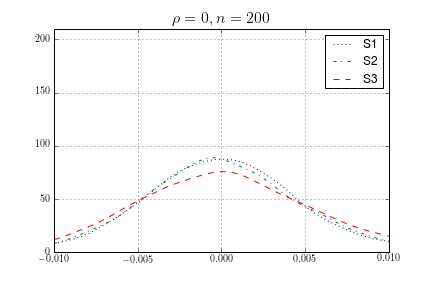
\includegraphics[width=8cm]{theta_density_200_0} & 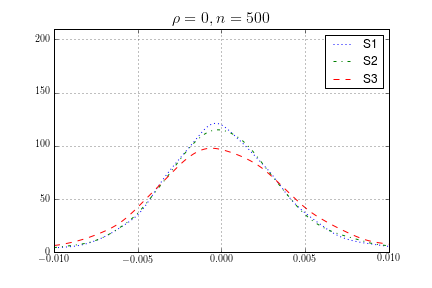
\includegraphics[width=8cm]{theta_density_500_0} \\
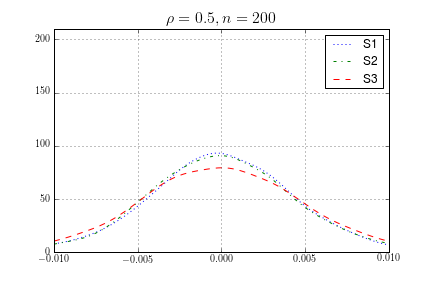
\includegraphics[width=8cm]{theta_density_200_05} & 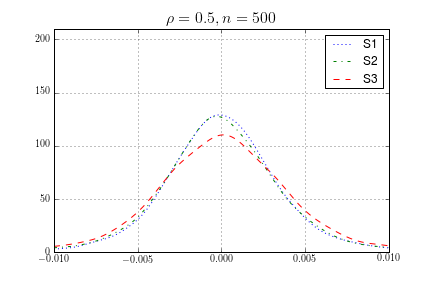
\includegraphics[width=8cm]{theta_density_500_05} \\
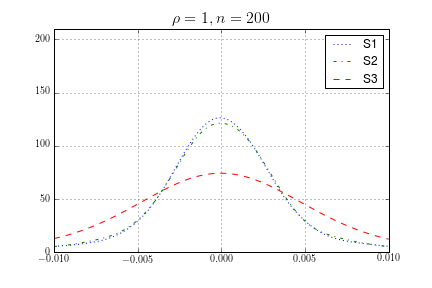
\includegraphics[width=8cm]{theta_density_200_1} & 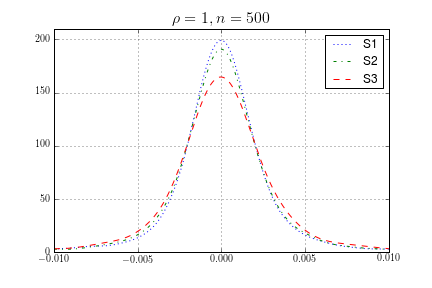
\includegraphics[width=8cm]{theta_density_500_1} \\
\end{tabular}
}
\end{table}



\clearpage

\begin{table}[!ht]
\selectfont \caption{Density estimate of $\hat{\al}_n$ (unscaled).}
\label{alpha_unscaled} \center{
\begin{tabular}{c c}
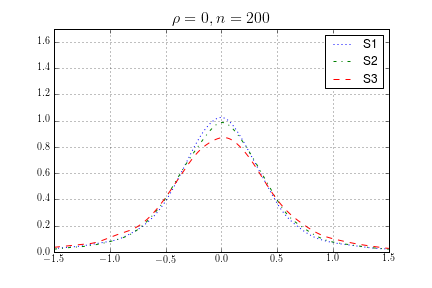
\includegraphics[width=8cm]{alpha_density_200_0} & 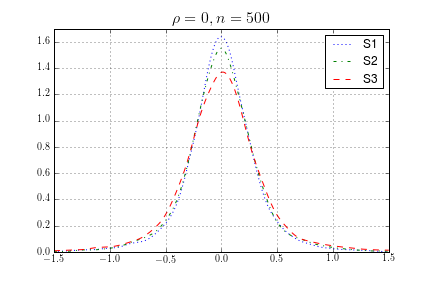
\includegraphics[width=8cm]{alpha_density_500_0} \\
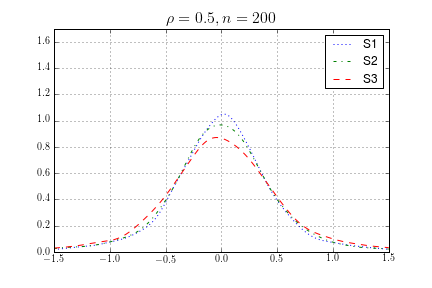
\includegraphics[width=8cm]{alpha_density_200_05} & 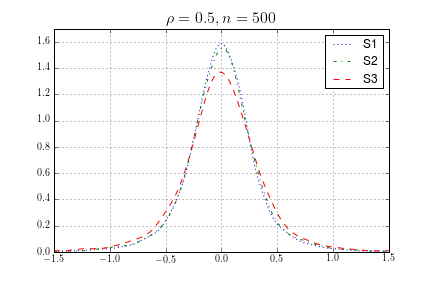
\includegraphics[width=8cm]{alpha_density_500_05} \\
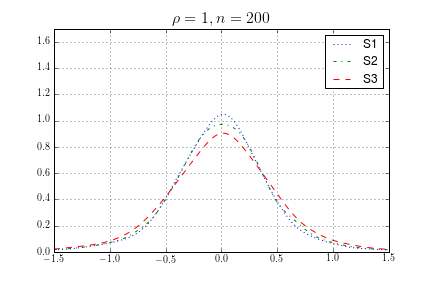
\includegraphics[width=8cm]{alpha_density_200_1} & 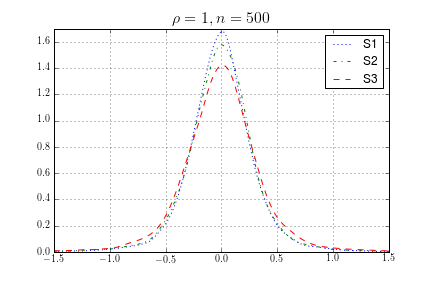
\includegraphics[width=8cm]{alpha_density_500_1} \\
\end{tabular}
}
\end{table}

\begin{table}[!ht]
\selectfont \caption{Density estimate of $\hat{\beta}_{1n}$ (unscaled).}
\label{beta1_unscaled} \center{
\begin{tabular}{c c}
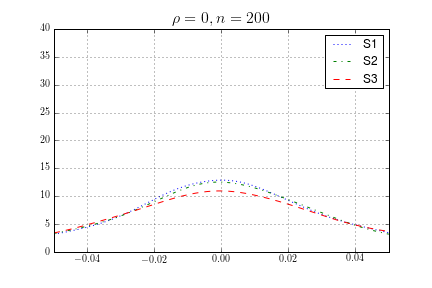
\includegraphics[width=8cm]{beta1_density_200_0} & 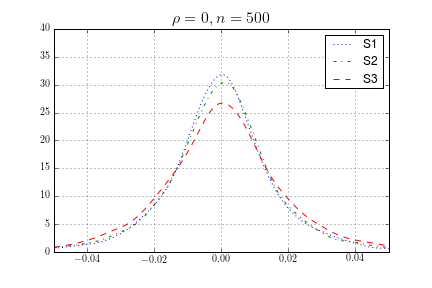
\includegraphics[width=8cm]{beta1_density_500_0} \\
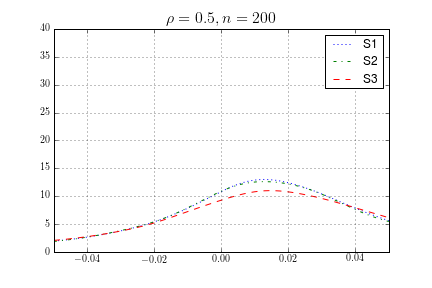
\includegraphics[width=8cm]{beta1_density_200_05} & 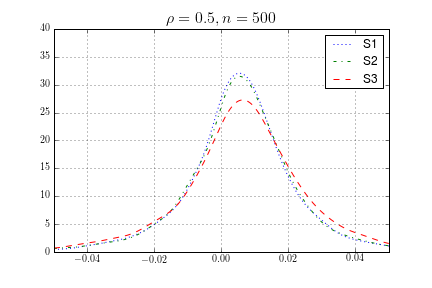
\includegraphics[width=8cm]{beta1_density_500_05} \\
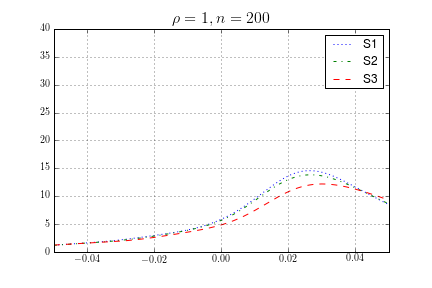
\includegraphics[width=8cm]{beta1_density_200_1} & 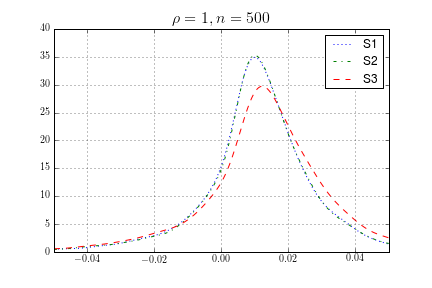
\includegraphics[width=8cm]{beta1_density_500_1} \\
\end{tabular}
}
\end{table}

\begin{table}[!ht]
\selectfont \caption{Density estimate of $\hat{\beta}_{2n}$ (unscaled).}
\label{beta2_unscaled} \center{
\begin{tabular}{c c}
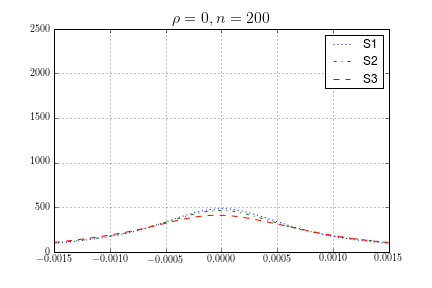
\includegraphics[width=8cm]{beta2_density_200_0} & 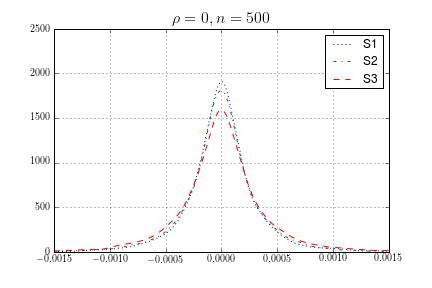
\includegraphics[width=8cm]{beta2_density_500_0} \\
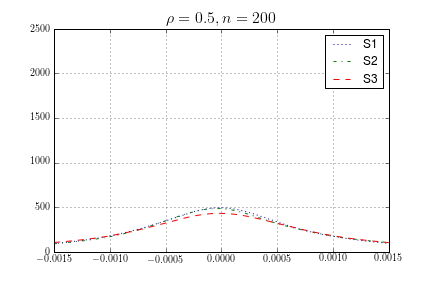
\includegraphics[width=8cm]{beta2_density_200_05} & 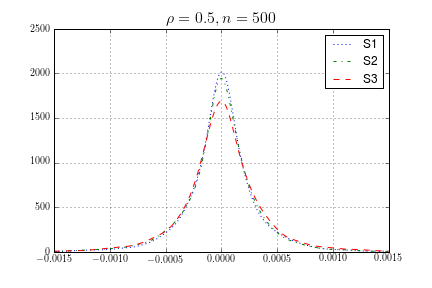
\includegraphics[width=8cm]{beta2_density_500_05} \\
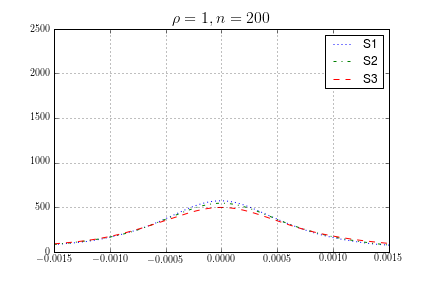
\includegraphics[width=8cm]{beta2_density_200_1} & 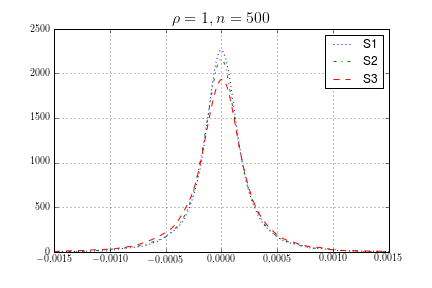
\includegraphics[width=8cm]{beta2_density_500_1} \\
\end{tabular}
}
\end{table}




\begin{table}[!ht]
\selectfont \caption{Density estimate of $\hat{\theta}_n$ (scaled by $n^{1/4}$).}
\label{theta_scaled} \center{
\begin{tabular}{c c}
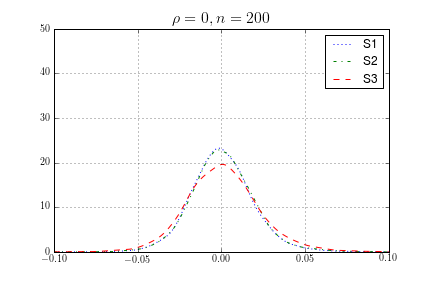
\includegraphics[width=8cm]{theta_scaled_density_200_0} & 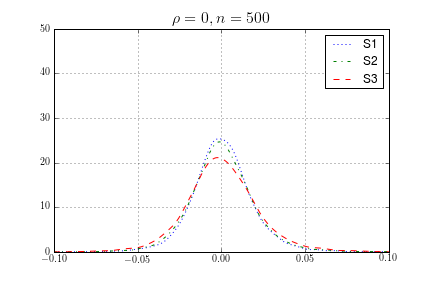
\includegraphics[width=8cm]{theta_scaled_density_500_0} \\
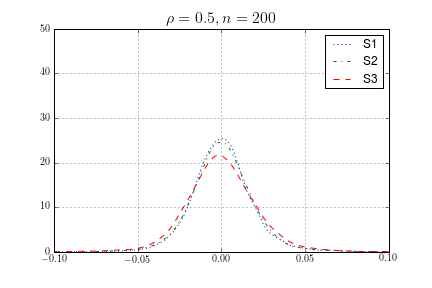
\includegraphics[width=8cm]{theta_scaled_density_200_05} & 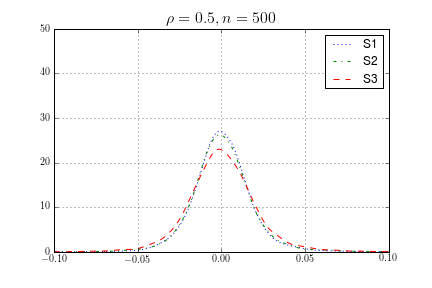
\includegraphics[width=8cm]{theta_scaled_density_500_05} \\
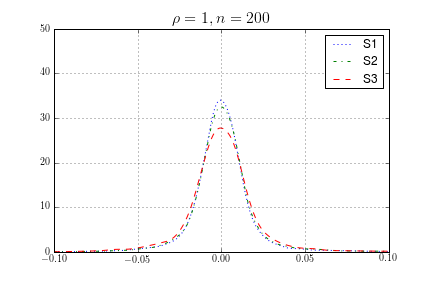
\includegraphics[width=8cm]{theta_scaled_density_200_1} & 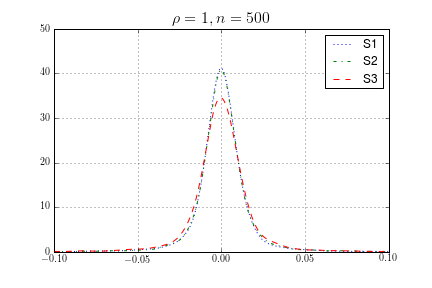
\includegraphics[width=8cm]{theta_scaled_density_500_1} \\
\end{tabular}
}
\end{table}




\begin{table}[!ht]
\selectfont \caption{Density estimate of $\hat{\alpha}_n$ (scaled by $n^{1/2}$).}
\label{alpha_scaled} \center{
\begin{tabular}{c c}
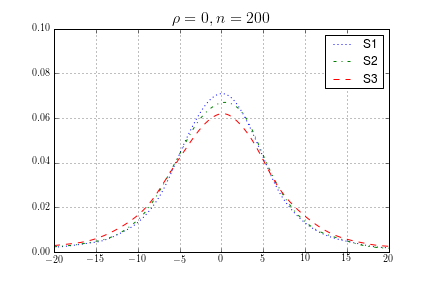
\includegraphics[width=8cm]{alpha_scaled_density_200_0} & 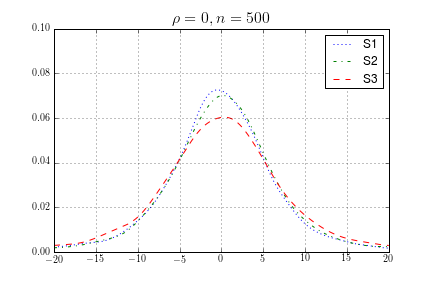
\includegraphics[width=8cm]{alpha_scaled_density_500_0} \\
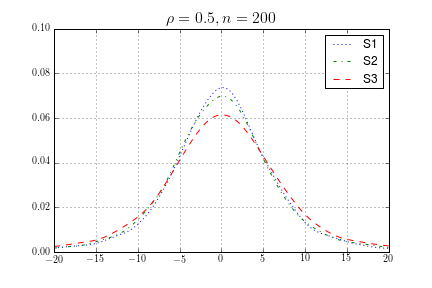
\includegraphics[width=8cm]{alpha_scaled_density_200_05} & 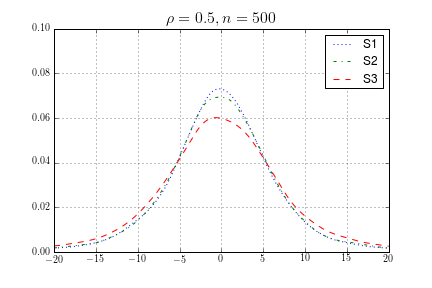
\includegraphics[width=8cm]{alpha_scaled_density_500_05} \\
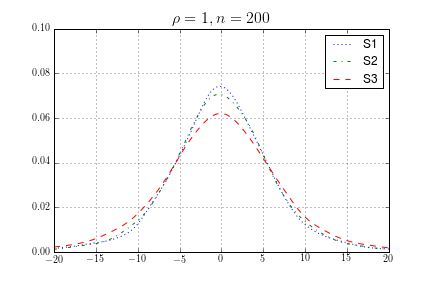
\includegraphics[width=8cm]{alpha_scaled_density_200_1} & 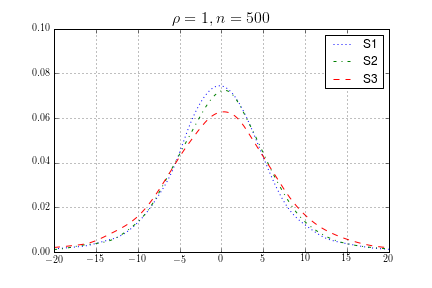
\includegraphics[width=8cm]{alpha_scaled_density_500_1} \\
\end{tabular}
}
\end{table}



\begin{table}[!ht]
\selectfont \caption{Density estimate of $\hat{\beta}_{1n}$ (scaled by $n$).}
\label{beta1_scaled} \center{
\begin{tabular}{c c}
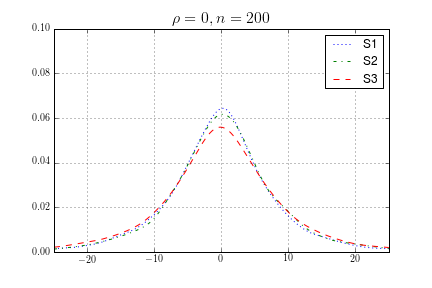
\includegraphics[width=8cm]{beta1_scaled_density_200_0} & 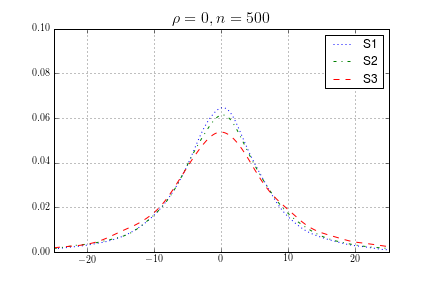
\includegraphics[width=8cm]{beta1_scaled_density_500_0} \\
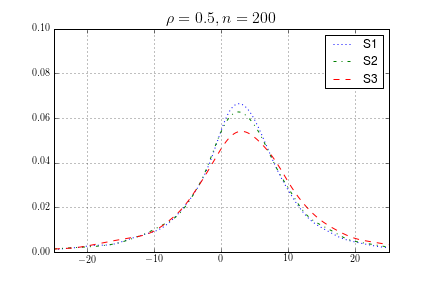
\includegraphics[width=8cm]{beta1_scaled_density_200_05} & 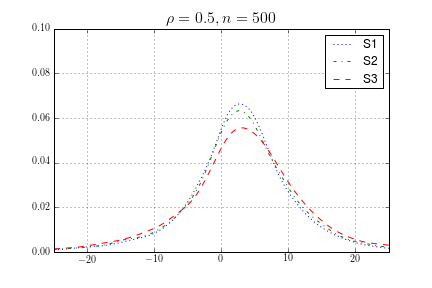
\includegraphics[width=8cm]{beta1_scaled_density_500_05} \\
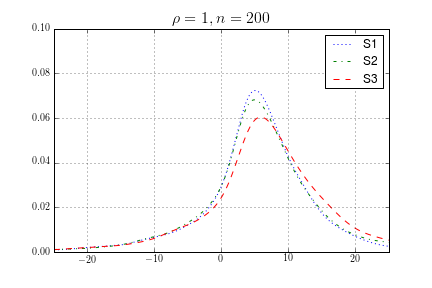
\includegraphics[width=8cm]{beta1_scaled_density_200_1} & 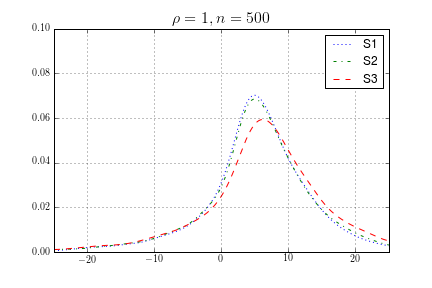
\includegraphics[width=8cm]{beta1_scaled_density_500_1} \\
\end{tabular}
}
\end{table}

\begin{table}[!ht]
\selectfont \caption{Density estimate of $\hat{\beta}_{2n}$ (scaled by $n^{3/2}$).}
\label{beta2_scaled} \center{
\begin{tabular}{c c}
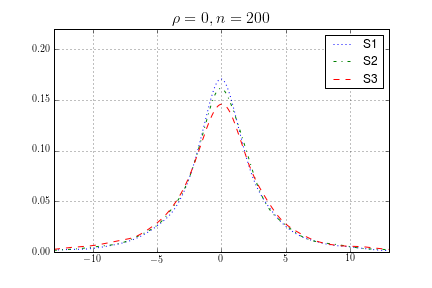
\includegraphics[width=8cm]{beta2_scaled_density_200_0} & 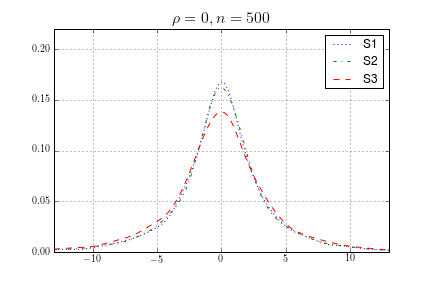
\includegraphics[width=8cm]{beta2_scaled_density_500_0} \\
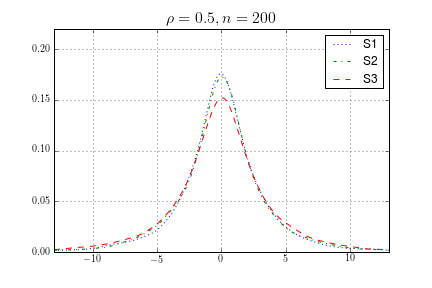
\includegraphics[width=8cm]{beta2_scaled_density_200_05} & 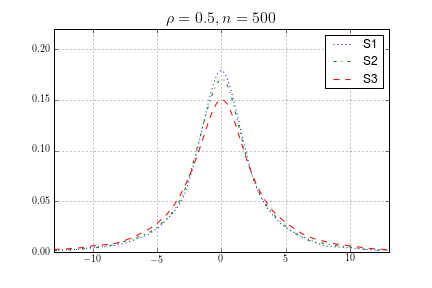
\includegraphics[width=8cm]{beta2_scaled_density_500_05} \\
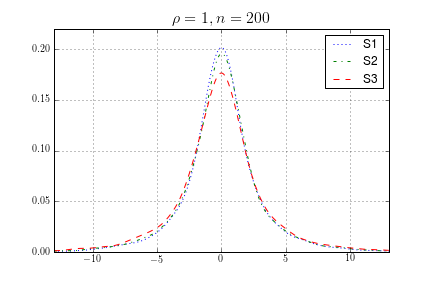
\includegraphics[width=8cm]{beta2_scaled_density_200_1} & 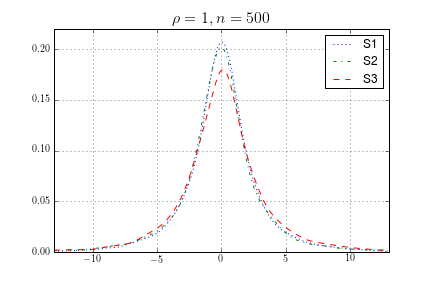
\includegraphics[width=8cm]{beta2_scaled_density_500_1} \\
\end{tabular}
}
\end{table}


\begin{table}[!ht]
\selectfont \caption{Density of $\hat{\theta}_n$ $t$-ratios.}
\label{theta_t} \center{
\begin{tabular}{c c}
\includegraphics[width=8cm]{theta_t_ratio_200_0} & \includegraphics[width=8cm]{theta_t_ratio_500_0} \\
\includegraphics[width=8cm]{theta_t_ratio_200_05} & \includegraphics[width=8cm]{theta_t_ratio_500_05} \\
\includegraphics[width=8cm]{theta_t_ratio_200_1} & \includegraphics[width=8cm]{theta_t_ratio_500_1} \\
\end{tabular}
}
\end{table}



\begin{table}[!ht]
\selectfont \caption{Density of $\hat{\alpha}_n$ $t$-ratios.}
\label{alpha_t} \center{
\begin{tabular}{c c}
\includegraphics[width=8cm]{alpha_t_ratio_200_0} & \includegraphics[width=8cm]{alpha_t_ratio_500_0} \\
\includegraphics[width=8cm]{alpha_t_ratio_200_05} & \includegraphics[width=8cm]{alpha_t_ratio_500_05} \\
\includegraphics[width=8cm]{alpha_t_ratio_200_1} & \includegraphics[width=8cm]{alpha_t_ratio_500_1} \\
\end{tabular}
}
\end{table}



\begin{table}[!ht]
\selectfont \caption{Density of $\hat{\beta}_{1n}$ $t$-ratios.}
\label{beta1_t} \center{
\begin{tabular}{c c}
\includegraphics[width=8cm]{beta1_t_ratio_200_0} & \includegraphics[width=8cm]{beta1_t_ratio_500_0} \\
\includegraphics[width=8cm]{beta1_t_ratio_200_05} & \includegraphics[width=8cm]{beta1_t_ratio_500_05} \\
\includegraphics[width=8cm]{beta1_t_ratio_200_1} & \includegraphics[width=8cm]{beta1_t_ratio_500_1} \\
\end{tabular}
}
\end{table}



\begin{table}[!ht]
\selectfont \caption{Density of $\hat{\beta}_{2n}$ $t$-ratios.}
\label{beta2_t} \center{
\begin{tabular}{c c}
\includegraphics[width=8cm]{beta2_t_ratio_200_0} & \includegraphics[width=8cm]{beta2_t_ratio_500_0} \\
\includegraphics[width=8cm]{beta2_t_ratio_200_05} & \includegraphics[width=8cm]{beta2_t_ratio_500_05} \\
\includegraphics[width=8cm]{beta2_t_ratio_200_1} & \includegraphics[width=8cm]{beta2_t_ratio_500_1} \\
\end{tabular}
}
\end{table}

\begin{table}[!ht]
\selectfont \caption{Estimate and 95\% Confidence Interval of $\hat{\al}_n$}
\label{alpha_plot} \center{
\begin{tabular}{c}
\includegraphics[width=16cm]{a_plot}
\end{tabular}
}
\end{table}

% \begin{table}[!ht]
% \selectfont \caption{Estmate and 95\% Confidence Interval of $\hat{\theta}_n = (\hat{\al}_n, \hat{\beta}_{1n}, \hat{\beta}_{2n})$}
% \label{GseqTable} \center{
% \begin{tabular}{c}
% %\includegraphics[width=16cm]{a_plot} \\
% \includegraphics[width=16cm]{b_1_plot} \\
% \includegraphics[width=16cm]{b_2_plot} \\
% \end{tabular}
% }
% \end{table}


\begin{table}[!ht]
\selectfont \caption{Confidence Intervals (95\% confidence) of $\hat{\alpha}_{n}$.}
\label{alpha_est} \center{
\begin{tabular}{|c |c  c  c|}
\hline
Country & $\hat{\alpha}_{n}$ & Lower & Upper \\
\hline
AUS & -57.387 & -58.005 & -56.769 \\
AUT & -25.352 & -26.414 & -24.290 \\
BEL & -41.632 & -43.144 & -40.121 \\
CAN & -44.442 & -45.615 & -43.268 \\
CHN & -32.402 & -38.126 & -26.678 \\
DEN & -113.670 & -115.375 & -111.965 \\
FIN & -91.869 & -94.019 & -89.720 \\
FRA & -76.449 & -78.162 & -74.735 \\
HOL & -71.892 & -73.439 & -70.344 \\
IND & -59.854 & -60.930 & -58.779 \\
IRE & -33.058 & -34.265 & -31.851 \\
ITA & -71.375 & -72.604 & -70.146 \\
JAP & -27.674 & -29.293 & -26.056 \\
NOR & -58.519 & -60.442 & -56.597 \\
USA & -45.950 & -46.945 & -44.954 \\
\hline
\end{tabular}
}
\end{table}



\begin{table}[!ht]
\selectfont \caption{Confidence Intervals (95\% confidence) of $\hat{\beta}_{1n}$.}
\label{beta1_est} \center{
\begin{tabular}{|c |c  c  c|}
\hline
Country & $\hat{\beta}_{1n}$ & Lower & Upper \\
\hline
AUS & 11.520 & 10.810 & 12.230 \\
AUT & 5.075 & 4.193 & 5.958 \\
BEL & 9.116 & 7.922 & 10.310 \\
CAN & 9.217 & 8.114 & 10.321 \\
CHN & 7.609 & 5.063 & 10.154 \\
DEN & 23.724 & 22.242 & 25.205 \\
FIN & 18.967 & 17.225 & 20.709 \\
FRA & 16.443 & 15.000 & 17.886 \\
HOL & 14.921 & 13.579 & 16.262 \\
IND & 14.908 & 13.894 & 15.923 \\
IRE & 6.816 & 6.062 & 7.570 \\
ITA & 14.502 & 13.647 & 15.356 \\
JAP & 5.447 & 4.614 & 6.279 \\
NOR & 11.802 & 10.555 & 13.050 \\
USA & 9.536 & 8.449 & 10.623 \\
\hline
\end{tabular}
}
\end{table}


\begin{table}[!ht]
\selectfont \caption{Confidence Intervals (95\% confidence) of $\hat{\beta}_{2n}$.}
\label{beta2_est} \center{
\begin{tabular}{|c |c  c  c|}
\hline
Country & $\hat{\beta}_{2n}$ & Lower & Upper \\
\hline
AUS & -0.562 & -0.730 & -0.394 \\
AUT & -0.246 & -0.389 & -0.102 \\
BEL & -0.485 & -0.721 & -0.248 \\
CAN & -0.462 & -0.732 & -0.192 \\
CHN & -0.446 & -0.775 & -0.118 \\
DEN & -1.226 & -1.586 & -0.865 \\
FIN & -0.967 & -1.256 & -0.678 \\
FRA & -0.875 & -1.190 & -0.559 \\
HOL & -0.762 & -1.093 & -0.432 \\
IND & -0.945 & -1.174 & -0.715 \\
IRE & -0.341 & -0.443 & -0.238 \\
ITA & -0.729 & -0.882 & -0.576 \\
JAP & -0.258 & -0.365 & -0.151 \\
NOR & -0.586 & -0.822 & -0.351 \\
USA & -0.477 & -0.768 & -0.186 \\
\hline
\end{tabular}
}
\end{table}



%%% Local Variables: 
%%% mode: latex
%%% TeX-master: "../thesis"
%%% End: 
